% LaTeX (version 2e) source for "LaTeX for Thesis and Large Documents"
% By Stephen Carr and Wail Gueaieb
% Updated 2005-04-07
%
% Parts to edit are marked by the following block:
%###################################
%## Edit this part
%###################################
% 
% Do NOT edit anything else unless you know what you are doing.
%
%======================================================================
%   P R E A M B L E
%======================================================================
\documentclass[%
12pt,   % font size
oneside,  % final version of thesis has to be submitted single-sided
%twoside, % in case you want to print a draft on both sides of the page
]{report}

%----------------------------------------------------------------------
%###################################
%## Edit this part
%###################################
\newcommand{\thesisauthor}{Philip D. Bulsink}
\newcommand{\thesistitlecoverpage}{%
  Exploring the Chemistry of Re$^I$:\\
  Physical and Theoretical Investigations
}
\newcommand{\thesistitleheadings}{\LaTeX for Thesis and Large Documents}
\newcommand{\degree}{Master of Science} 
\newcommand{\nameofprogram}{Chemistry}
\newcommand{\academicunit}{Ottawa-Carleton Chemistry Institute}
\newcommand{\graduationyear}{2014}
\newcommand{\supervisors}{Professors Darrin Richeson \& Tom Woo}

\newcommand{\abstractfile}{abstract.tex}
\newcommand{\acknowledgementfile}{acknowledgement.tex}
%----------------------------------------------------------------------
% Reprocess only those files which have changed recently:
%\includeonly{intro,creating,commands} 
%----------------------------------------------------------------------
% Create a listing in the log of all files needed to process this document
\listfiles
%----------------------------------------------------------------------
\makeindex % activate index-making
%----------------------------------------------------------------------
% THESIS PREAMBLE
% By Stephen Carr and Wail Gueaieb
% Updated 2005-04-07

% The following command sets "1.2" as the line spacing throughout the
% thesis for readability (optional).
\renewcommand{\baselinestretch}{1.2}
%----------------------------------------------------------------------
% Reset page margins properly for doublesided pages
\usepackage[letterpaper,includehead,left=3.25cm,right=2.5cm,top=2.5cm,headsep=1.5cm,headheight=0.0cm,bottom=2.5cm,footskip=1.0cm]{geometry} 
% \setlength{\marginparwidth}{0pt}
% \setlength{\marginparsep}{0pt}
% \setlength{\oddsidemargin}{0.125in}
% \setlength{\evensidemargin}{0.125in}
% \setlength{\textwidth}{6.375in}
\raggedbottom
%----------------------------------------------------------------------
%%%%%%%%%%%%%%%%%%%%%%%%%%%%%%%%%%%%%%%%%%%%%%%%%%%%%%%%%%%%%
 % thesis-specific settings
%----------------------------------------------------------------------
% My own command and environment definitions:
\newcommand{\program}[1]{\textbf{#1}} % program names in bold text
\newcommand{\exten}[1]{\texttt{#1}} % file extensions in bold text (use caps)
\newcommand{\cmmd}[1]{\textbackslash\texttt{#1}} % command name in tt font 
\newcommand{\enviro}[1]{\texttt{#1}} % environment name in tt font

\newcommand{\eg}{\textit{e.g.},} % some Latin abreviations in italic
\newcommand{\ie}{\textit{i.e.},}
\newcommand{\etc}{\textit{etc}.\@}

\newcommand{\mat}[1]{\ensuremath{\mathcal{#1}}} 
	% matrix names in uppercase caligraphic
\newcommand{\vect}[1]{\ensuremath{\mathit{#1}}} 
% vector names in math italic
\newcommand{\rv}[1]{\ensuremath{\mathbf{#1}}} 
% math bold for random variables
\newcommand{\degg}[1]{\mbox{\raisebox{3pt}{$\circ$}\hspace{-.5pt}#1}}
% command to produce a degree sign. Example: \degg[C] gives degrees Celcius

\newenvironment{definition}[1]{\begin{quote}\emph{#1}:}{\end{quote}}
  % Provides indented formal definition and emphasizes the word.
  % e.g. \begin{definition}{Reliability} ... \end{definition}

\newenvironment{where}[1]% Equation symbol lists
 {\begin{list}{}%
  {\renewcommand{\makelabel}[1]{\hfill\textnormal{##1 =}}%
   \settowidth{\labelwidth}{\textnormal{#1 =}}%
   \setlength{\leftmargin}{\labelwidth}%
   \addtolength{\leftmargin}{\labelsep}%
   \setlength{\itemsep}{-\parsep}}}%
 {\end{list}}
% Example:
% \begin{where}{where $E$}
%  \item[where $E$] least squares error term;
%  \item[$w$] weighting factor associated with each measured variable.
% \end{where}
\renewcommand{\thefootnote}{\roman{footnote}}
%----------------------------------------------------------------------
% Standard LaTeX2e packages I am using (as seen in "The LaTeX Companion"):
\usepackage[]{graphicx} 
	% ... if you want to include encapsulated postscript figures
%\usepackage{makeidx} % ... if you want an index
%\usepackage{amsmath} % ... if you need lots of math symbols
\usepackage[bookmarks=true,linktocpage]{hyperref} % ... only needed for PDF generation
\usepackage{setspace}
\usepackage{fixltx2e}
\usepackage[backend=bibtex,style=chem-acs,biblabel=dot]{biblatex}
\addbibresource{bibliography/thesis}
\usepackage[labelfont=bf, labelsep=space, tableposition=top]{caption}
\usepackage{chemscheme}
%\usepackage[varioref=false]{chemstyle}
\usepackage[version=3]{mhchem}

\usepackage[nonumberlist, toc, nopostdot]{glossaries}
\renewcommand\glossaryname{Glossary of Terms}
\makeglossaries

\newacronym{ac.tga}{TGA}{Thermogravimetric Analysis}
\newacronym{ac.dft}{DFT}{Density Functional Theorem}
\newacronym{ac.tddft}{TD-DFT}{Time Dependant Density Functional Theorem}
\newacronym{ac.nmr}{NMR}{Nuclear Magnetic Resonance}
\newacronym{ac.homo}{HOMO}{Highest Occupied Molecular Orbital}
\newacronym{ac.lumo}{LUMO}{Lowest Unoccupied Molecular Orbital}
\newacronym{ac.mlct}{MLCT}{Metal-Ligand Charge Transfer}
\newacronym{ac.dmf}{DMF}{N,N-dimethylformamide}
\newacronym{ac.teoa}{TEOA}{Triethanolamine}
\newacronym{ac.tea}{TEA}{Triethylamine}

\usepackage{booktabs}
\usepackage[textwidth=2.8cm]{todonotes}
\setlength{\marginparwidth}{2.8cm}
\reversemarginpar

\usepackage{float}
\floatstyle{plaintop}
\restylefloat{table}

\usepackage{pdflscape}
\usepackage{afterpage}
\usepackage{subcaption}
\usepackage{multirow}
\usepackage[para]{threeparttable}


\usepackage[section]{placeins}


\usepackage{fancyvrb}
%----------------------------------------------------------------------
% Non-standard packages I am using (things I've written, borrowed, etc.):
%\usepackage{} % ... note that old .sty files can be included here

%======================================================================
%   L O G I C A L    D O C U M E N T
%======================================================================
\begin{document}
%----------------------------------------------------------------------
% FRONT MATERIAL
%----------------------------------------------------------------------
% TITLE PAGE 
% By Stephen Carr and Wail Gueaieb
% Updated 2005-04-07

\pagestyle{empty} % No headers or page numbers

\begin{center}

\vspace*{1.0cm}
{\bf \LARGE %
  \thesistitlecoverpage}

\vspace*{1.0cm}
\normalsize
by \\
\vspace*{1.0cm}
\Large
\thesisauthor\\
\vspace*{2.0cm}
\normalsize
Thesis submitted to the\\
Faculty of Graduate and Postdoctoral Studies\\
In partial fulfillment of the requirements\\
For the \degree~degree in\\
\nameofprogram\\

\vspace*{2.0cm}
\academicunit\\
\faculty\\
University of Ottawa\\

\vspace*{2.0cm}
\copyright~\thesisauthor, Ottawa, Canada, \graduationyear\\

\end{center}

\newpage
 
%%%%%%%%%%%%%%%%%%%%%%%%%%%%%%%%%%%%%%%%%%%%%%%%%%%%%%%%%%%%%

% PRELIMINARY PAGES
\pagestyle{plain} % No headers, just page numbers
\pagenumbering{roman} % Roman numerals
\setcounter{page}{2}

%----------------------------------------------------------------------
% This page is not needed for the University of Ottawa
% % Declaration Page
% \noindent
% I hereby declare that I am the sole author of this thesis.

% \noindent
% I authorize the University of Ottawa to lend this thesis to other
% institutions or individuals for the purpose of scholarly research.
% \vspace{4cm}

% \noindent
% \thesisauthor

% \vspace{4cm}

% \noindent
% I further authorize the University of Ottawa to reproduce this thesis by
% photocopying or other means, in total or in part, at the request of other
% institutions or individuals for the purpose of scholarly research.
% \vspace{4cm}

% \noindent
% \thesisauthor
% \newpage
%----------------------------------------------------------------------

% Long abstract (manually formatted)
\begin{center}
\Large
\textbf{Abstract}
\end{center}
\input{\abstractfile}
\newpage

% Acknowledgements and/or Dedication Pages
\begin{center}\textbf{Acknowledgements}\end{center}
\input{\acknowledgementfile}
\newpage

% Pages which are generated automatically
\setcounter{page}{6} % Set this counter to get correct page numbers
\tableofcontents
\listoftables
\listoffigures
\newpage

% Change page numbering back to Arabic numerals
\pagenumbering{arabic}
%%%%%%%%%%%%%%%%%%%%%%%%%%%%%%%%%%%%%%%%%%%%%%%%%%%%%%%%%%%%%
 
% Title page, declaration, borrowers' page, abstract, acknowlegements, 
% dedication, table of contents, list of tables, list of figures

%----------------------------------------------------------------------
% MAIN BODY
%----------------------------------------------------------------------
% HEADINGS 
% By Stephen Carr and Wail Gueaieb
% Updated 2005-04-07

% Put the document title and page numbers in the header
%\pagestyle{headings}
\pagestyle{myheadings}
% Put title on left & chapter heading goes on right by default
\markboth{\thesistitleheadings}
% Go to normal sized type
\normalsize


 % Specify thesis headings
%----------------------------------------------------------------------
%###################################
%## Edit this part
%###################################
% Chapters 
% Include your "sub" source files here (must have extension .tex)
\doublespacing
\chapter{Introduction}
\markright{Introduction} % new right header
%======================================================================
\section{Inorganic Chemistry}
%======================================================================

Common distinctions split most chemical compounds into one of two categories: organic and inorganic. Organic molecules contain carbon and hydrogen, with or without additional nitrogen, oxygen, phosphorus, sulfur, and the halides. Inorganic chemistry is, therefore, considered to be the remainder of the molecules possible. While they may include come aspect of organic chemistry (especially in organometallic molecules), the main structural motif or reactive center is a non-organic feature. These inorganic compounds can range from compounds such as lithium or grignard reagents with significant organic influence, to metallic alloys or mineral compounds. With such a wide range of possibilities, inorganic chemistry has many facets. A widely active research area is the development and testing of transition metal complexes for catalytic, photo-physical, biochemical or manufacturing uses.

%======================================================================
\section{Photochemistry \& Catalysis}
%======================================================================

A report of the first synthesized organometallic complex was published by Zeise in 1831\autocite{zeise1831}. To form what is now known as Zeise's salt, K[PtCl\textsubscript{3}(C\textsubscript{2}H\textsubscript{4})].H\textsubscript{2}O,he mixed platinum chloride with ethanol, followed by a reaction with potassium chloride\autocite{hunt1984}. After some controversy to the composition of this, it was confirmed by Griess and Martius\autocite{griess1861}, and later expanded upon by Birnbaum\autocite{birnbaum1868}. 

The field of organometallics was expanded greatly by Frankland, and many of his complexes were catalytically active. Further development of this new chemistry quickly led to useful catalysts for the conversion of petroleum products or the production or destruction of other chemicals to be developed using nearly all of the transition metals. These catalysts take all forms, from simple olefin and halide compounds to multi-metallic complexes with large organic ligands.

Some of the most interesting organometallic catalysts since the late 1990s have been the development of earth metal pincer complexes to replace noble metal or early transition metal catalysts, which are often more toxic or expensive to produce. Brookhart and Gibson published a series of papers\autocite{small1998a, small1998b, britovsek1998, britovsek1999} on the use of iron and cobalt with bis-imino pyridine ligands to perform ethylene polymerization at rates exceeding those of similar noble metal complexes and metallocenes\autocite{gibson2007}. The role of the ligand in the mechanism is still up for debate, but many modified systems have been synthesized and tested since the first work was published\autocite{boudier2014}.

Many of these types of pincer complexes are photochemically active. In transition metal complexes, the interaction between the metal atom(s) and the ligands can cause significant electron mobility upon the absorption of incident photons. The metal atom's \textit{d} orbitals typically lie at or near the highest occupied molecular orbital (HOMO) energy, while the ligands often have low energy anti-bonding orbitals ($\pi^\ast$) at the lowest unoccupied molecular orbital (LUMO) levels. When a photon is absorbed and is promoted from the ground state to the excited state, that state is geographically removed from the metal centre, this motion of the electron is labelled a metal-ligand charge transfer (MLCT). Formally, the metal atom is oxidized by the photons, this oxidation allows for redox reactivity at the metal centre for as long as the electron remains removed to the ligand. Relaxation (through photon emission via fluorescence or phosphorescence, or via vibrational or other motion processes) can return the electron to the metal to reform the ground electronic state. 



%======================================================================
\section{Rhenium}
%======================================================================

Rhenium compounds display a broad scope of applications ranging from catalysis\autocite{dudle2011, jain2008, kuninobu2011} to radiopharmaceutical applications\autocite{bartholoma2009, schibli2002}, as well as possessing interesting fundamental photophysical properties\autocite{coogan2009}. Since the mid-1970's, complexes containing the $\alpha$-diimine Re\textsuperscript{I} tricarbonyl core have attracted a great deal of attention due to their attractive photochemical properties with pseudo-octahedral \textit{fac}-[L\textsubscript{2}Re(CO)\textsubscript{3}X] and \textit{fac}-[L\textsubscript{2}(L')Re(CO)\textsubscript{3}]\textsuperscript{+} complexes being the dominant species\autocite{giordano1979, fredericks1979, sacksteder1990, caspar1983, yam2001, feliz1998, ruiz1996, lin1992, hino1992, walters2002, striplin2001}. A large family of compounds with these formulations have been accessed by the addition of chelating diimine $\sigma$-donor ligands to [Re(CO)\textsubscript{5}X] with the quantitative replacement of two \textit{cis} carbonyls in the Re\textsuperscript{I} starting material\autocite{giordano1979, martin2011, abel1959, kirkham1965, zingales1967, gamelin1994, marti2005, morse1976, giordano1978}. Significantly, these reactions form only bidentate coordinated ligands with \textit{facial} tricarbonyl isomers as products even when a potentially tridentate $\sigma$-donor, such as bis(imino)pyridine or 2,2':6',2''-terpyridine are employed in the reaction (Figure \ref{fig.terdentateligands})\autocite{granifo1999, orrell1997, abel1993}. These robust species have been examined for potential applications in organic light-emitting diodes (OLEDs)\autocite{gong1998}, chemosensors and biotechnology probes\autocite{lo2010, lin2007, slone1995, beer1999, beer2003}, fluorescence microscopy imaging of cells\autocite{lo2010, amoroso2008, amoroso2007}, and the photochemical reduction of CO\textsubscript{2} to CO\autocite{hawecker1983, hawecker1986, takeda2010, christensen1992, sullivan1985}. Among the key photophysical features of these $\alpha$-diimine Re\textsuperscript{I} compounds is the electron transfer capability of this system and the interplay between the Re center and the well-known non-innocent redox-activity of the ligands\autocite{caulton2012}.

\begin{figure}[!htbp]
 \begin{center}
  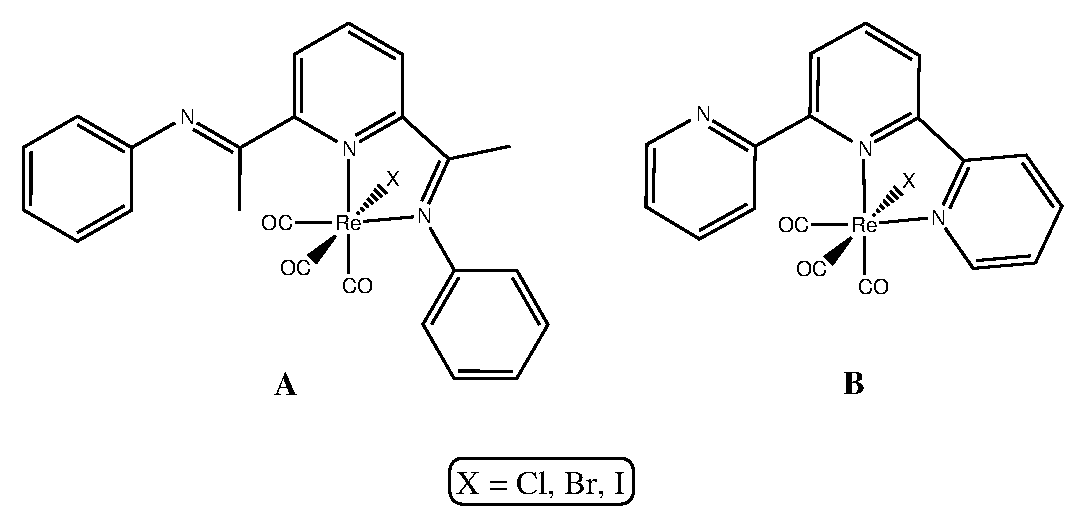
\includegraphics[clip=true, width=110mm]{images/terdentateligands.eps}
 \end{center}
\caption[Two common bidentate complexes using terdentate ligands]{Two common \textit{fac}-[L\textsubscript{2}Re(CO)\textsubscript{3}X] complexes with terdentate $\sigma$-donor ligands: L = bis(imino)pyridine (\textbf{A}) and 2,2':6',2''-terpyridine (\textbf{B})}
\label{fig.terdentateligands}
\end{figure}

Further development of this chemistry has been restricted by the limited structural and electronic variability of the common pseudo-octahedral \textit{fac}-[L\textsubscript{2}ReX(CO)\textsubscript{3}] (L\textsubscript{2} = $/alpha$-diimine) products. While these systems continue to receive considerable attention, studies detailing the coordination chemistry of the meridionally-coordinated tridentate triimine Re\textsuperscript{I} dicarbonyl core are quite limited\autocite{jurca2013}. For example, while $\kappa$\textsubscript{3}-(terpy)Re(CO)\textsubscript{2}Cl was initially reported in 1988\autocite{juris1988}, closer analysis of the reported analytical data (including \textsuperscript{1}H NMR) indicate that this compound is more likely $\kappa$\textsubscript{2}-LRe(CO)\textsubscript{3}Cl. A more recent report for this compound provides spectroscopic details of this species as well as the preliminary report for the generation of [($\kappa$\textsubscript{3}-(terpy)Re(CO)\textsubscript{2}L’]\textsuperscript{+} cations (L = PPh\textsubscript{3}, PEt\textsubscript{3}, NC\textsubscript{5}H\textsubscript{5}, and NCCH\textsubscript{3})\autocite{black2012}. Finally, the \textsuperscript{1}H NMR data for ($\kappa$\textsubscript{3}-(terpy)Re(CO)\textsubscript{2}Br) has been reported\autocite{abel1993}.

In order to fully exploit the potential of this versatile family of compounds, the limits imposed by the bidentate coordination need to be addressed. Furthermore, it would appear that, on the basis of the tridentate ligands that have been investigated, the concerted effort to produce the tridentate species has been unsuccessful. Attracted by this challenge we sought to synthesize, crystallographically authenticate, and investigate the photophysical properties of low-valent rhenium pincer complexes displaying an N,N',N''-chelated terpyridine array. 

We recently reported the conversion of bidentate bis(imino)pyridine complexes 2,6-\{2,6-Me\textsubscript{2}C\textsubscript{6}H\textsubscript{3}N=CPh\}\textsubscript{2}(NC\textsubscript{5}H\textsubscript{3})Re(CO)\textsubscript{3}X  (X = Cl, Br) into tridentate pincer ligand compounds, 2,6-\{2,6-Me\textsubscript{2}C\textsubscript{6}H\textsubscript{3}N=CPh\}\textsubscript{2}(NC\textsubscript{5}H\textsubscript{3})Re(CO)\textsubscript{2}X (X = Cl, Br)\autocite{jurca2013}. This transformation was performed in the solid-state by controlled heating of these bidentate species above 200$^\circ$C in a tube furnace under a flow of nitrogen gas giving excellent yields ($\geq$~95\%). These compounds defined a new coordination environment for Re\textsuperscript{I} carbonyl chemistry where the metal center is supported by a planar, tridentate pincer coordinated bis(imino)pyridine ligand. 

Complexes of 2,2':6',2''-terpyridine (terpy) are of interest due to the conceptual relationship to established bis(imino)pyridine compounds\autocite{russell2010, tondreau2012}. Herein, we provide rational synthetic procedures to these novel species as well as their characterization and analysis of their visible electronic transitions. These results will broaden the accessibility of such compounds for investigation and application. This report for the unconventional but accessible synthesis of tridentate pincer complexes promises to enhance the versatile chemistry of Re\textsuperscript{I} and yield new venues for exploration.

This thesis will be a discussion of the development of chemistry of Re\textsuperscript{I} complexes, their characterization, and comparison of structural and photo-physical properties to computed values. Further exploration of the CO\textsubscript{2} reduction by photo-catalysis of these new complexes will be analyzed. This thesis will also take a more detailed look at specifics of the mechanisms proposed for current Re\textsuperscript{I} diimine catalysts, and propose new geometries for prior mechanistic steps based on experimental, computational, and literature review work.

 %"Organometallic, Photochem & catalysis, rhenium"
\chapter{New Coordination Geometries for \texorpdfstring{\ce{Re^I}}{Rhenium (I)}}
\markright{New Coordination Geometries for \texorpdfstring{\ce{Re^I}}{Rhenium (I)}} % new right header
%======================================================================
\section{Introduction}
%======================================================================

As mentioned previously in the thesis introduction, \ce{Re^I} compounds have been typically bidentate (\ce{$\kappa$^2}) compounds, even when using a potentially terdentate (\ce{$\kappa$^3}) ligand such as bis(imino)pyridine or terpyridine (refer to \autoref{fig.terdentateligands}). The chemistry of this rhenium $\alpha$-imino complex has been extensively invesigated, with over 1700 references appearing in a structure search for that metal-ligand motif. The extraction of an additional carbonyl and the chelation of the pendant arm of the ligand was attempted to extend the pi system of the ligand and its interaction with the metal centre. This was first demonstrated by prior work in our group for the bis(imino)pyridine ligand\autocite{jurca2013}. 

%======================================================================
\section{Synthesis of Bidentate and Terdentate}
%======================================================================

Similar to the prior work, synthesis began with the production of bidentate \ce{$\kappa$2(terpy)Re(CO)3X} (X = Cl, Br) by coordination of 2,2':6',2''-terpyridine (Sigma) with a \ce{Re(CO)5X} (Strem) starting material in dry toluene at reflux for 4 hours. A bright yellow powder precipitated from solution and was collected by filtration, washed with cold hexanes, and dried \textit{in vacuo} to a good yield\footnote{Experimental details for all compounds can be seen in \nameref{chap:appA}}. These bidentate compounds were used without further purification to produce \ce{$\kappa$3(terpy)Re(CO)2X} (X = Cl, Br) via thermolysis. 

%======================================================================
\section{Anion Exchange}
%======================================================================


%======================================================================
\section{Characterization}
%======================================================================

%----------------------------------------------------------------------
\subsection{NMR Analysis}
%----------------------------------------------------------------------

%----------------------------------------------------------------------
\subsection{X-Ray Crystallography}
%----------------------------------------------------------------------

%----------------------------------------------------------------------
\subsection{Spectroscopy}
%----------------------------------------------------------------------

% - - - - - - - - - - - - - - - - - - - - - - - - - - - - - - - - - - -
\subsubsection{Infrared Spectroscopy}
% - - - - - - - - - - - - - - - - - - - - - - - - - - - - - - - - - - -

% - - - - - - - - - - - - - - - - - - - - - - - - - - - - - - - - - - -
\subsubsection{UV-Vis Spectroscopy}
% - - - - - - - - - - - - - - - - - - - - - - - - - - - - - - - - - - -

%----------------------------------------------------------------------
\subsection{Conclusions}
%----------------------------------------------------------------------

 %"new geometry chemistry"
%======================================================================
\chapter{Photocatalysis of \texorpdfstring{CO\textsubscript{2}}{CO2}}\label{chap.co2}
\markright{Photocatalysis of \texorpdfstring{CO\textsubscript{2}}{CO2}}
%======================================================================

%======================================================================
\section{Introduction}
%======================================================================

Only 6 years after \ce{Re^I} complexes using 2,2'-bipyridine were characterized, Hawecker, Lehn, and Ziessel showed the effectiveness of the compound for the photocatalytic reduction of \ce{CO2}\autocite{hawecker1983}. Since then, many have shown the efficacy of a wide range of $\alpha$-diimino complexes for the reaction\autocite{hawecker1986, kurz2006, portenkirchner2014} and expansion of the systems to bimetallic complexes with ruthenium and osmium as electron transfer agents has produced a wide range of results\autocite{rossenaar1996, takeda2008, tamaki2013}. The mechanism of reduction has been subject of some debate: while mechanisms have been proposed since Lehn et. al. soon after their original publication\autocite{hawecker1986}, modifications have been submitted routinely over the past decades\autocite{hayashi2003, morris2009, takeda2008, grills2010, agarwal2011, agarwal2012a, agarwal2012b, keith2013}. The development of a novel terdentate geometry and the associated increase in photon absorption at lower energies of the catalyst warranted investigation of the \ce{CO2} reduction capabilities, having overcome the criticism of only utilizing high energy photons \autocite{kutal1985}. 

%======================================================================
\section{Photocatalytic Reactions with New Compounds}
%======================================================================

The photocatalytic cycle is, simply, a photon-induced \gls{ac.mlct}, followed by the extraction of an electron from a sacrificial reductant. This radical, negatively charged species sheds the anion, opening up a reaction site. Reaction between a \ce{CO2}, a proton (from the decomposition of the reductant or elsewhere), and the catalyst yields any number of \ce{CO}, \ce{H2O}, formate (\ce{HCO2-}), or carbonate (\ce{CO3H-}), depending on the mechanistic pathway. Further discussion and a proposal of a new mechanism geometry based on computational and experimental data can be read in \autoref{chap.mech}.

%----------------------------------------------------------------------
\subsection{Conditions}
%----------------------------------------------------------------------

Reaction conditions in use in literature have remained typically unchanged since the original papers. A mixture of \gls{ac.dmf} with either \gls{ac.teoa} or \gls{ac.tea} at a 5:1 ratio is used to make a 1.0 mM solution of catalyst, with `excess' (depending on reference, a 1.1 to 25 molar ratio) electrolyte salt (typically \ce{Et4NX} or \textit{t}-\ce{Bu4NX}, where X = halide from catalyst) added as a stabilizer. Solutions are degassed by bubbling of \ce{CO2} and a consistent headspace is left to form over the solution. The reaction is monitored via \gls{ac.gc} analysis of the headspace, using a HP gas chromatograph with a 15 m CARBONPLOT column with 0.320 mm inner diameter and 1.50 $\mu$m film in a 40~$^\circ$C oven. The instrument is fitted with a \gls{ac.tcd}, and, while using He as a carrier gas, is able to resolve \ce{CO} and \ce{CO2} completely.  

%----------------------------------------------------------------------
\subsection{Experimental Results}
%----------------------------------------------------------------------

Both bidentate and terdentate \ce{$\kappa$^n(terpy)Re(CO)_{5-n}X} (n=2, 3) \textbf{2.1} and \textbf{2.2} complexes show no activity for \ce{CO2} reduction. Modification of testing time, light source, product analysis methods, solvent, sacrificial reductant, pH, presence of electrolyte, presence of \ce{H2O}, or variation of anion (X=Cl, Br, OTf, CN) shows no change of this inactivity. Testing of \ce{$\kappa$^2(bipy)Re(CO)3Cl} under the same reaction and testing conditions shows production of approximately 6 mL \ce{CO} from \ce{CO2} (~20\% conversion) in 1 hour of photolysis with visible ($\lambda$ \textgreater 400 nm) light, verifying the method, isolating the catalyst as the ineffective species. 

%======================================================================
\subsection{Rationalization of Results}\label{ss.rationalization}
%======================================================================
\todo{TEOA insertion, maybe clear is a acid, formate, carbonate, tricarbonylcation or other complex?}

Kurz \textit{et al.} demonstrated the requirement for fluorescence for successful catalytic candidates\autocite{kurz2006}. The explanation for this is the requirement for a stable, long-lasting excited state, with lifetime greater than that of the timescale required for electron abstraction from the sacrificial amine. The observed fluorescence demonstrates the lack of non-radiative relaxation pathways, considered to be an analogue for the extended lifetime of the excited state. Sample \textbf{2.2} shows only poor fluorescence. While the complex is able to absorb light across the spectrum, and has \gls{ac.homo} to \gls{ac.lumo} transitions with high enough energy\footnote{Electrochemical reduction of \ce{CO2} in similar environments takes 1.7-2.1 V, equivalent to \gls{ac.homo}-\gls{ac.lumo} transitions from 590-750 nm\autocite{grills2014}.} for the catalyzed reduction of \ce{CO2} to \ce{CO}, it appears as if the catalysis is not initiated due to a short excited state lifetime. Fluorescence data presented in \autoref{chap.newchem}, at \autoref{ss.fluorescence} shows the lack of strong fluorescence in terdentate sample \textbf{2.2}.

Explanation for the lack of \ce{CO} production observed in the attempted photochemical reduction of \ce{CO2} by bidentate sample \textbf{2.1} and others must come from another angle. These samples are quite fluorescent, emission from the powder sample can be seen with the naked eye with simulation by a 405 nm laser pen under ambient light environments. Importantly, two clues come from the reaction mixture: under intense visible light in the presence of \ce{CO2} the compound bleaches to a very faint yellow-green and colour does not return after storage in the dark, bubbling of new \ce{CO2}, or other manipulations. Secondly, a mixture of sacrificial amine, \gls{ac.dmf}, and catalyst \textbf{2.1} in ratios identical to what is required in the reaction mixture changes colour from a yellow to a deep red irreversibly after 5 days at ambient temperature.

\begin{scheme}[!htb]
 \begin{center}
  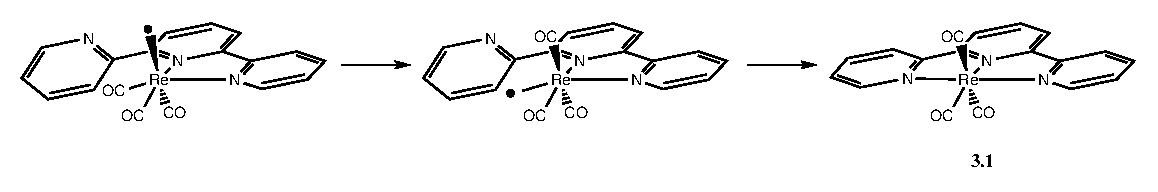
\includegraphics[clip=true, width=120mm, keepaspectratio]{images/tricarbscheme.eps}
 \end{center}
\caption[Reorganization from catalytic eximer to form \textbf{3.1}]{Formation of \textbf{3.1} from catalytic excimer via reorganization of carbonyls and chelation of the pendant arm.}
\label{scheme.tricarbonyl}
\end{scheme}

\todo{The most likely cause of bleaching is due to ligand loss. }

The appearance of the irreversible red product may be the formation of triethanolamine-catalyst adducts\autocite{morimoto2013}. In the presence of DMF, TEOA has been shown to bind to the open site of the excimer via the amine's oxygen atom. This is susceptible to insertion of \ce{CO2} to form a --\ce{OC(O)C}--\ce{CH2CH2N(CH2CH2OH)2} group. \Gls{ac.dft} studies on these two compounds suggest that they may be a coloured species, with predicted UV-Vis showing lower energy absorption than the catalyst itself (a red shift), demonstrated in \autoref{fig.ishitani}.

\begin{figure}[!htbp]
 \begin{center}
  \includegraphics[clip=true, keepaspectratio, width=120mm]{images/ishitani.eps}
 \end{center}
\caption[UV-Vis spectra for \textbf{2.1} and catalyst-TEOA complex]{Computational structure (inset) and \gls{ac.dft} predicted UV-Vis absorption spectra for \textbf{2.1} (blue) and the \gls{ac.teoa} complex proposed by Ishitani\autoref{fig.ishitani} (red)}
\label{fig.ishitani}
\end{figure}

\todo{ishitani figure}






 %"CO2 Chemistry" 
%======================================================================
\chapter{Mechanism of \texorpdfstring{CO\textsubscript{2}}{CO2} Reduction}
\markright{Computational Study of the Mechanism of \texorpdfstring{CO\textsubscript{2}}{CO2} Reduction}
%======================================================================
Text
%======================================================================
\section{Section}
%======================================================================
\subsection{Subsection}
%----------------------------------------------------------------------

%----------------------------------------------------------------------
\subsection{Subsection}
%----------------------------------------------------------------------

%----------------------------------------------------------------------
\subsection{Subsection}
%----------------------------------------------------------------------

% - - - - - - - - - - - - - - - - - - - - - - - - - - - - - - - - - - - 
\subsubsection{SubSubSection}
% - - - - - - - - - - - - - - - - - - - - - - - - - - - - - - - - - - -

% - - - - - - - - - - - - - - - - - - - - - - - - - - - - - - - - - - -
\subsubsection{SubSubSection}
% - - - - - - - - - - - - - - - - - - - - - - - - - - - - - - - - - - -

% - - - - - - - - - - - - - - - - - - - - - - - - - - - - - - - - - - -
\subsubsection{SubSubSection}
% - - - - - - - - - - - - - - - - - - - - - - - - - - - - - - - - - - -

%======================================================================
\section{Section}
%======================================================================

%======================================================================
\section{Section}
%======================================================================

%----------------------------------------------------------------------
\subsection{Subsection}
%----------------------------------------------------------------------
 %"Mechanism Study"
%======================================================================
\chapter{TurboControl}\label{chap.turbocontrol}
\markright{TurboControl}
%======================================================================

Elucidation of the mechanism using computational methods required a significant amount of manual set-up and analysis work of computational input and output files. The calculations required hundreds different molecules, intermediates, or transition state candidates to be calculated in multiple different environments, with the final mechanism employing 38 species in gas and solvated systems. These calculations typically require analyst intervention or set-up of intermediate steps to be able to fully elucidate all of the required information. For example, frequency calculations must be set up after a geometry optimization to ensure ground state or transition state geometries. 

Additionally, while TurboMole contains much faster optimization code for \gls{ac.dft} calculations, the user interface is exceptionally user-unfriendly and involves an abrasive interactive text prompt environment. This contrasts to Gaussian~09, which is significantly more popular, particularly due to the user-friendliness of the GaussView \gls{ac.gui}, despite concerns about the speed of optimization of large or complex molecules.

These two factors prompted the development of a new program, TurboControl, written in Python, with the goal of combining the user friendliness of GaussView on top of the optimization efficiency of TurboMole. This program allows a user to prepare the input files in GaussView, modify them slightly in any text editor available to them, then run a batch calculation on the files. TurboControl monitors the computational jobs, resubmitting for frequency calculations when optimization is complete if requested, and using the TurboMole tools available when required to ensure ground state or first transition state geometries are discovered. TurboControl then creates a single output file, providing the energy and first frequency vibration of each molecule. Additional commands can instruct TurboControl to run molecules in a simulated solution, do single-point energy calculations, or gather more in-depth thermodynamic information from the outputs using TurboMole's tools. 

TurboControl provides this hands-off management of jobs allowing the user to spend more time in data analysis, experimental work, or to be able to produce data at a significantly higher rate compared to the manual setup and monitoring of jobs. TurboControl also contains a single job initiation script entitled TurboGo to allow for the use of the input files without the prior experience with turbomole.

This section will describe the development, features and usage of the TurboControl code in more detail. 

%----------------------------------------------------------------------
\section{Development}
%----------------------------------------------------------------------

TurboControl began as a script for the simple setup and submission of jobs in TurboMole from Gaussian input files. The jobs were submitted to the `wooki' computing cluster managed by the Woo lab, available at the University of Ottawa. This computing cluster consists of approximately 1000 CPU cores, running the CentOS distribution of Linux available in the Rocks software distribution. The GridEngine queuing system ensures fair usage of computing cores for each user, and maximizes throughput by managing computational jobs. 

TurboControl initially submitted jobs and monitored their successful completion or failure. Development quickly expanded to include automatic resubmission for frequency analysis of geometry optimization jobs, required to determine the success of finding an energy minima (stationary point) instead of a transition state. TurboMole contains multiple ways of determining the ground state frequency of a geometry optimized molecule, TurboControl is granular enough to utilize whichever method is requested, or will default to a particular method if none is requested explicitly. While some methods are parallel calculations in TurboMole, others are able to utilize only a single processor core. Resubmitting jobs to the cluster's queue after each step ensures computational resources are not wasted, they are able to be shared appropriately by the queue.

As the complexity of the mechanistic study (see \autoref{chap.mech}) increased to include analysis of thermodynamic data, calculation of transition states, calculation in solution phases, and more, the capabilities of TurboControl were developed to meet these increased demands. 

TurboControl is now able to handle large batches of input, with jobs of varying complexity and monitor them through successful completion or failure of the TurboMole calculation. Analysis of the computational jobs is performed to simply highlight \gls{ac.dft} energies, first computed normal mode frequencies, and thermodynamic properties (if requested).  

Development of TurboControl contained extensive testing at every step. Each function was tested as extensively as possible, including edge cases, error cases, and null inputs. This testing minimizes runtime errors, reducing the frequency of crashes of the code. Some code was unable to be subjected to programmed testing, the code interacting with the TurboMole scripts directly has been tested manually by developing test use cases. Test coverage can be seen in \autoref{app.readme}, \nameref{sec.code}.

Code was written to be `object oriented', that is, the code treats every molecule and job as an object, with defined properties, functions, and methods to manipulate these objects. This is a well defined coding style utilized when dealing with many items of similar type that contain data, when that object can be manipulated, activated, or modified. The data in the object is not modified directly, changes to the data is accessed via methods that are properties of the object.

The code was written to be compliant with popular best practices, particularly those designed for the Python language and described in `PEP8'\autocite{pep8}. Deviations from the style guide were minimized and permitted only in special cases. Proper in code documentation was included as well, using both docstrings and inline comments\autocite{pep257}. This ensures code readability and simplifies future development by any author. The entire project is approximately 5500 lines of code, including tests, helper scripts, licence, and readme files. 

%----------------------------------------------------------------------
\section{Usage}
%----------------------------------------------------------------------

TurboControl is available freely on the internet, and is a fully open-source project\autocite{bulsink2014}. The code may be downloaded by anyone and be installed and used without prior permission for personal, academic, or commercial purposes, provided that the original software license remains with the code. TurboControl works only with the stated versions of software in the `readme' file available with the code on the internet (and included in \autoref{app.readme}). The software requires no installation prior to use, and has very few dependencies beyond the typically installed packages on a Unix or Linux system. 

TurboControl and TurboGo are not quantum mechanical packages themselves, they require a properly licensed installation of TurboMole to perform calculations. Additionally, while GaussView may be used to prepare the input files, modification of the files by hand in a text editor is required to access most features, GaussView is not required for the use of TurboControl. 

%----------------------------------------------------------------------
\section{Conclusions}
%----------------------------------------------------------------------

TurboControl and TurboGo are two scripts developed to maximize throughput and minimize operator involvement in large computational studies utilizing TurboMole. Development of these scripts is not limited to the scope of the thesis, an open source licence and source code freely available on the internet mean this project may be adopted and further developed by others who are interested in its use. The scripts are not quantum chemical packages themselves, a fully licensed copy of the TurboMole software is required for their usage.


 %"Turbocontrol"
%======================================================================
\chapter{Conclusions}
\markright{Conclusions}
%======================================================================

The target \ce{Re^I} terdentate terpyridine compounds were successfully synthesized and fully characterized. The experiments resulted in the first crystalographically verified \textit{mer}-$\kappa^3$-(N, N', N'')-\ce{Re(CO)2X} complexes. These terpyridine complexes are accessed via a simple, highly efficient, solid-state thermolysis pathway. These complexes expand the previously known $\alpha$-diimino photophysical properties, with enhanced metal-to-ligand d-$\pi^\ast$ electronic transitions than the associated bidentate compounds. These experimental observations are supported by computational \gls{ac.tddft} results, providing  a deeper understanding of frontier molecular orbital environments for these complexes. 

The synthesized catalysts were tested for the photoreduction of \ce{CO2}. The $\alpha$-triimino catalysts show no activity for the reduction of \ce{CO2}, in contrast to the known excellent bipyridine compounds, potentially due to the lack of fluorescence of the terdentate complexes, and the chelating ability of the pendant arm in the bidentate 2,2':6,2''-terpyridine ligand. These catalysts may be suitable for electrocatalytic reduction of \ce{CO2}, further investigation will be required.

Reaction mechanisms of the photocatalytic reduction of \ce{CO2} by bipyridine catalysts were studied successfully with \gls{ac.dft} methods, resulting in the proposed new geometry for the production of {CO} with no carbonate or formate anions. This new geometry does not conflict with known experimental studies, yet avoids three-body mechanistic steps previously seen in literature. This geometry provides explanation for previously unexplained phenomenon of \ce{^{13}CO} ligand exchange in few turnovers.

Development of a tool for the rapid submission and automated job monitoring for the TurboMole program facilitated the mechanism investigation by maximizing computational throughput while minimizing set-up and analysis time for the user. The scripts increase the `black box' nature of TurboMole, increasing the usability to include those unfamiliar with the program, and take advantage of the high performance of TurboMole relative to other computational suites. An open source licence and freely available source code mean this project may continue with other developers in the future



 %"Conclusion"
%----------------------------------------------------------------------
% END MATERIAL
%----------------------------------------------------------------------
%###################################
%## Edit this part
%###################################
% Appendices
\appendix
\captionsetup{list=no}
% Designate with \appendix declaration which just changes numbering style 
% from here on
%\include{useful_pkgs} %"Some Useful \LaTeX2e Packages"
%\include{appendix1-help} %"Sources of Information and Help"
% An appendix
%======================================================================
\chapter{Experimental Procedures}\label{chap.exp}
\markright{Experimental Procedures}
%======================================================================

Experimental synthesis and characterization data for the compounds discussed in this thesis are shown below by compound number:

\section{General Methods}\label{sec:.genmethods}
Synthesis reactions were set-up in a glovebox under a nitrogen atmosphere and performed under an inert atmosphere. Solvents were sparged with nitrogen and then dried by passage through a column of activated alumina using an apparatus purchased from Anhydrous Engineering. Deuterated chloroform and deuterated acetonitrile was dried using activated molecular sieves. Rhenium starting materials were purchased from Strem Chemicals and used as received. All other chemicals were purchased from Aldrich and used without further purification. \Gls{ac.nmr} spectra were run on Bruker Avance 400MHz spectrometers with \ce{CD3CN} or \ce{CDCl3} as solvent and internal standard. Elemental analyses were performed by Midwest Microlab LLC, Indianapolis IN. Solid state reactions were carried out in a Lindberg Blue M Mini-Mite Tube Furnace (model TF55035A-1). Infrared spectra were collected using an Agilent Technologies Cary FT-IR spectrometer using a diamond ATR attachment. UV-Vis spectra were collected using a Agilent Technologies Cary 5000 UV-Vis spectrometer. \Gls{ac.tga} was performed on a TA Q5000 IR instrument: approximately 10-15~mg of each sample was placed in a ceramic sample pan which was heated at a rate of 5~$^\circ$C/min up to 150~$^\circ$C, followed by a rate of 2~$^\circ$CC/min to 300~$^\circ$C while being purged with \ce{N2} at a flow rate of 25~mL/min. \Gls{ac.gc} was performed using a HP gas chromatograph with a 15 m CARBONPLOT column with 0.320 mm inner diameter and 1.50~$\mu$ film in a 40~$^\circ$C oven. The instrument is fitted with a \gls{ac.tcd} at 220~$^\circ$C.

\section{Computational Methods}\label{sec.compmethods}
For the UV-Vis and experimental correlation study, the structures of all species were optimized using Gaussian 09\autocite{gaussian} employing the B3LYP\autocite{becke1993, lee1988}  exchange-correlation (XC) functional. The LanL2DZ basis set/effective core potential\autocite{hay1985} was used on Re and, the all-electron TZVP basis set\autocite{schafer1994} for the remaining lighter atoms. Frequency analysis of all structures was used to confirm the nature of the stationary points. Solvent effects were computed using the integral equation formalism variant of the PCM solvation model within Gaussian 09 for both the ground state and excited state TD-DFT calculations with DMSO as the solvent\autocite{tomasi2005, scalmani2006}. The UV-Vis absorption spectra were extracted using the Chemissian software\autocite{chemissian}. In these calculations, a pseudo-Voigt band shape was employed with a default average band width at half-height of 2000cm\ce{^{-1}}.

For the mechanism study, the ground and transition state structures and energies of all species were obtained by using TurboMole 6.5 software\autocite{turbomole, ahlrichs1989} with the TPSS meta-GGA XC functional\autocite{tao2003}. The def2-TZVP basis set was used for all atoms\autocite{schafer1994, weigend2005}. The TurboMole program contains a number of optimizations to the original \gls{ac.dft} algorithms\autocite{haase1993, treutler1995, eichkorn1997, eichkorn1995, sierka2003, deglmann2004, weigend2002, vonarnim1998, ahlrichs2004}, decreasing the calculation time without compromising accuracy. Grimme's dispersion correction (version 3) was included in the calculations\autocite{grimme2010}. Intermediates and transition states were verified by frequency analysis\autocite{deglmann2004, deglmann2002, grimme2002}. The effects of solvation was calculated using the Conductor-like Screening Model (COSMO) implemented in TurboMole\autocite{klamt1993}, which is a continuum solvation model implicitly surrounding the solute molecule.

\section{X-ray Crystallography}\label{sec.xray}
Crystals were mounted on thin glass fibers using paraffin oil. Prior to data collection crystals were cooled to 200.15K. Data were collected on a Bruker AXS SMART single crystal diffractometer equipped with a sealed Mo tube source (wavelength 0.71073 \r{A}) APEX II CCD detector. Raw data collection and processing were performed with APEX II software package from BRUKER AXS53. Diffraction data for sample \textbf{3} was collected with a sequence of 0.5$^\circ$ $\omega$ scans at 0, 120, and 240$^\circ$ in $\phi$. Due to lower unit cell symmetry in order to ensure adequate data redundancy, diffraction data for \textbf{1}, \textbf{2} and \textbf{8} were collected with a sequence of 0.5$^\circ$ $\omega$ scans at 0, 90, 180 and 270$^\circ$ in $\phi$. Initial unit cell parameters were determined from 60 data frames with 0.3$^\circ$ $\omega$ scan each collected at the different sections of the Ewald sphere. Semi-empirical absorption corrections based on equivalent reflections were applied\autocite{blessing1995}. Systematic absences in the diffraction data-set and unit-cell parameters were consistent with triclinic P$\overline{1}$ ($\mathcal{N} ^\mathcal{O}$2) for compounds \textbf{1}, \textbf{2} and \textbf{8}, monoclinic \textbf{C}2/c ($\mathcal{N} ^\mathcal{O}$15) for compound \textbf{3}. Solutions in the centrosymmetric space groups for all compounds yielded chemically reasonable and computationally stable results of refinement. The structures were solved by direct methods, completed with difference Fourier synthesis, and refined with full-matrix least-squares procedures based on $F^2$.

Solutions for \textbf{1} and \textbf{2} revealed that both these structures contain two compound molecules per asymmetric unit.

Initial refinement results for the compound \textbf{1} suggested presence of two non-merohedrally twinned domains. Two independent orientation matrices were found using CELL\textunderscore NOW software\autocite{cellnow}. Data set was re-integrated with two independent orientation matrices and consecutive model refinement was performed using HKLF5 format reflection data file. Twinning domain ratio coefficient (BASF) was successfully refined to 0.3794.

On the final model refinement stage for compound \textbf{2} thermal motion parameters for coordinated CO (-C(33)=O(3)) and Cl (Cl(2)) moieties as well as presence of unusually strong residual electron density peaks in one of the compound molecules suggested a positional CO / Cl disorder not related by symmetry. Disorder was successfully modeled with refined occupation ratio at one position CO / Cl = 70\%:30\%. Disorder of the second position was inversed in such way that overall occupancy summed up to one full CO and one full Cl ligands in the first coordination sphere of Re metal center. Set of geometrical (SADI) and thermal motion (SIMU, DELU) restrains were applied to achieve acceptable molecular fragment geometries and thermal motion parameter values.

For all the compounds hydrogen atoms positions were initially assigned from the residual electron density peaks coordinates. However, after initial placement all hydrogen atoms were treated as idealized contributions during the refinement. All scattering factors are contained in several versions of the SHELXTL program library, with the latest version used being v.6.12\autocite{sheldrick2008}.

\subsection{X-Ray Structures from Multiple Vantage Points}\label{ssec.views}
Multiple views of each x-ray structure (including full unit cell) as discussed in \autoref{chap.newchem} are shown in \Cref{fig.xray21,fig.xray22,fig.xray23,fig.xray25,fig.xray28}. 

\begin{figure}[!ht]
 \centering
 \begin{subfigure}[b]{0.49\textwidth}
  \includegraphics[clip=true, width=\textwidth, height=50mm, keepaspectratio]{images/xray1a.eps}
 \end{subfigure}
 \begin{subfigure}[b]{0.49\textwidth}
  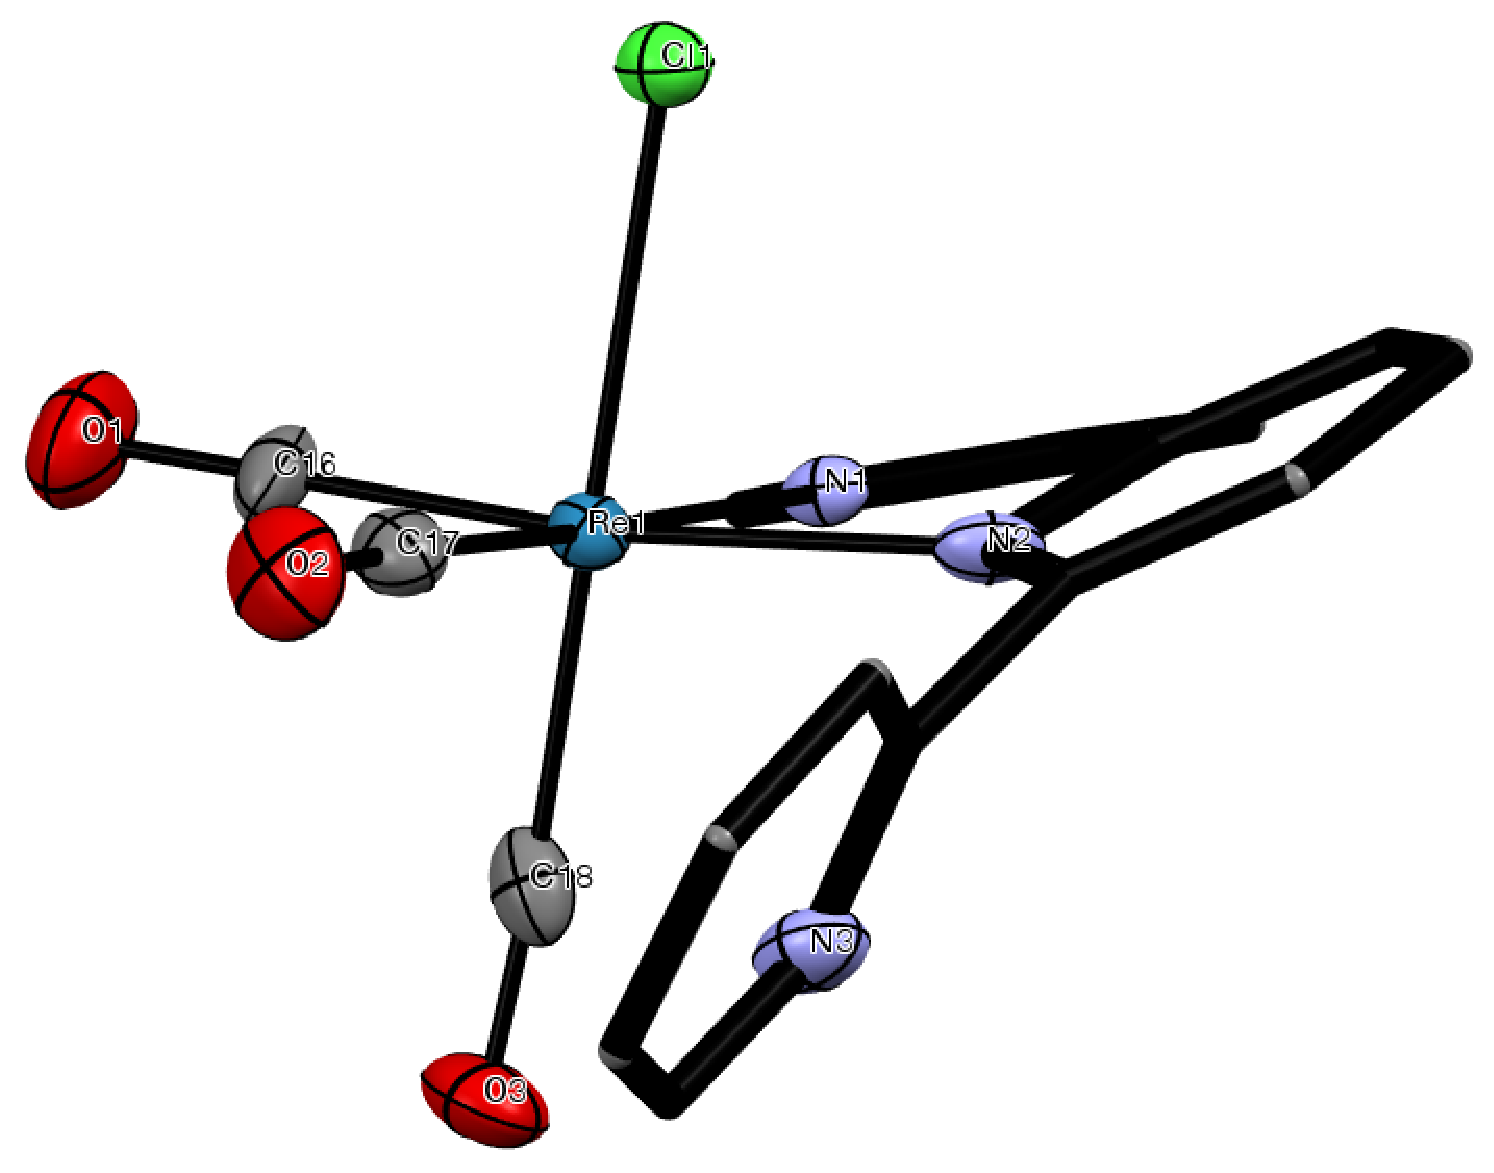
\includegraphics[clip=true, width=\textwidth, height=50mm, keepaspectratio]{images/xray1b.eps}
 \end{subfigure}
 \begin{subfigure}[b]{0.49\textwidth}
  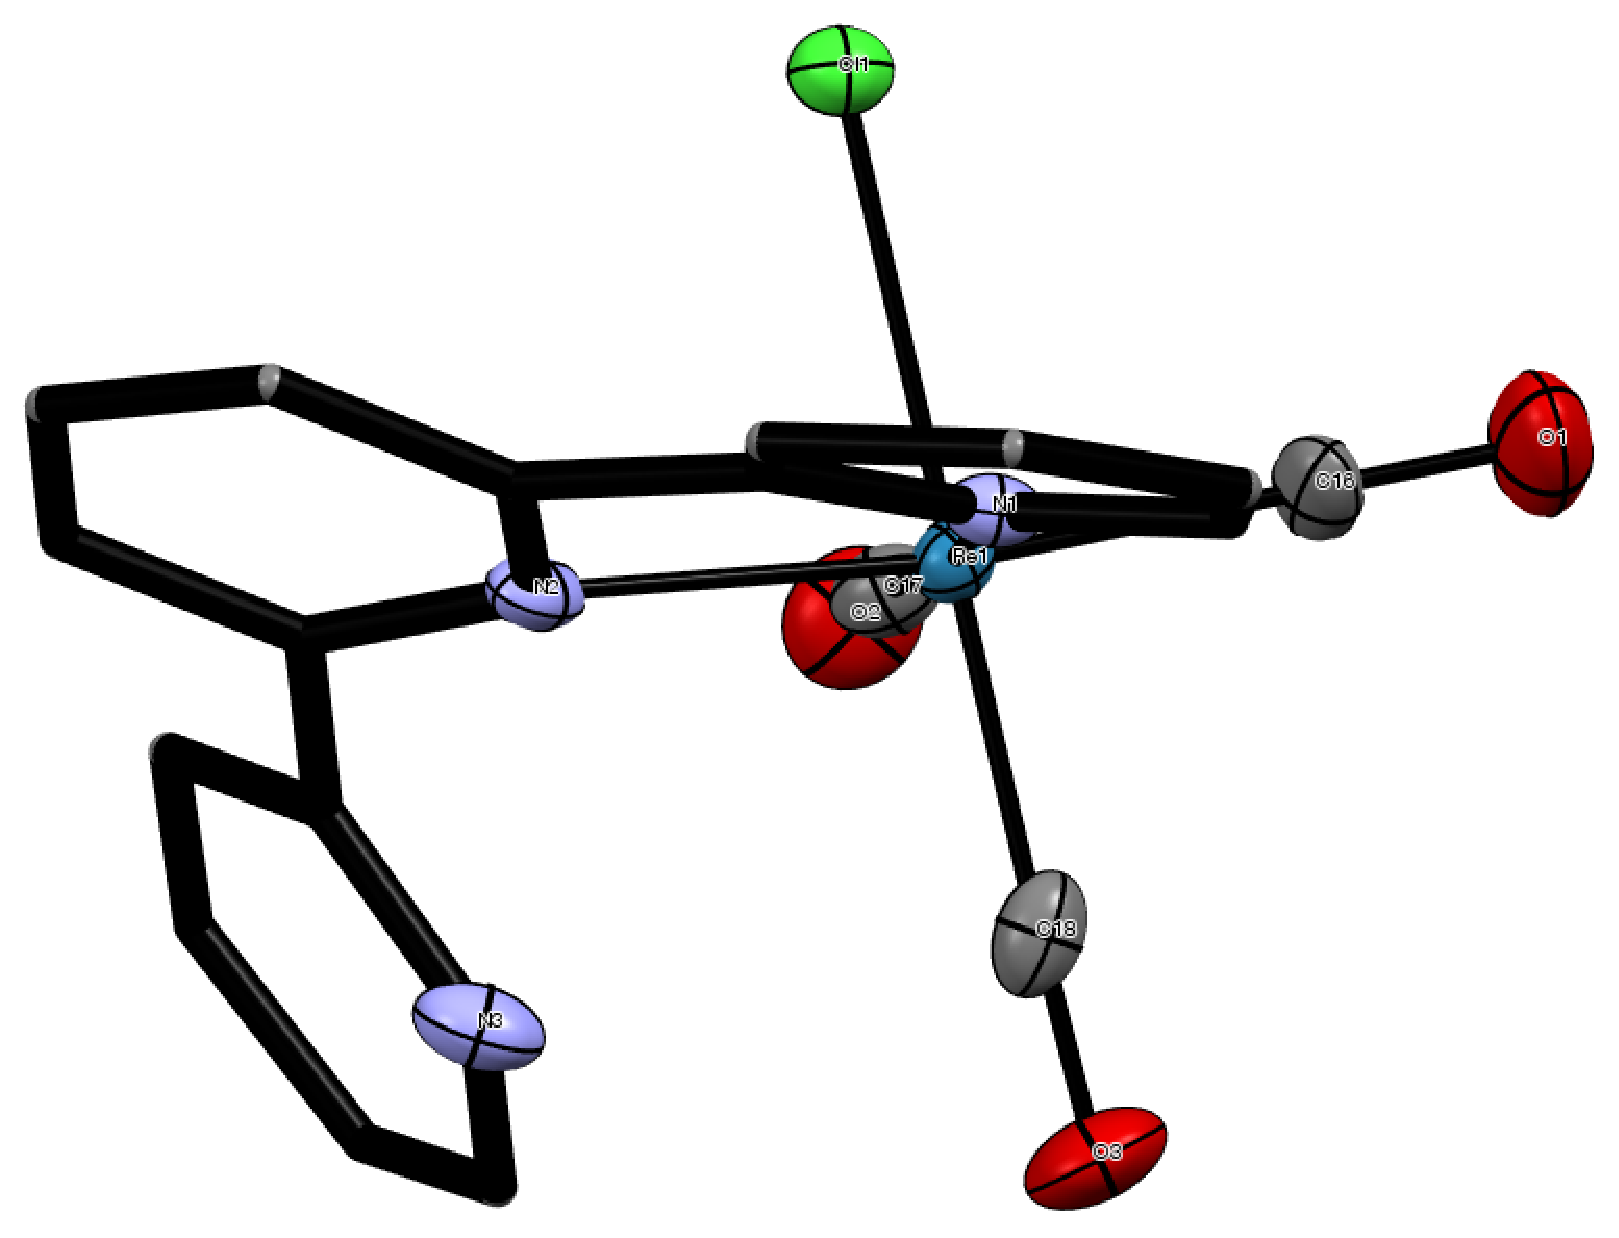
\includegraphics[clip=true, width=\textwidth, height=50mm, keepaspectratio]{images/xray1c.eps}
 \end{subfigure}
  \begin{subfigure}[b]{0.49\textwidth}
  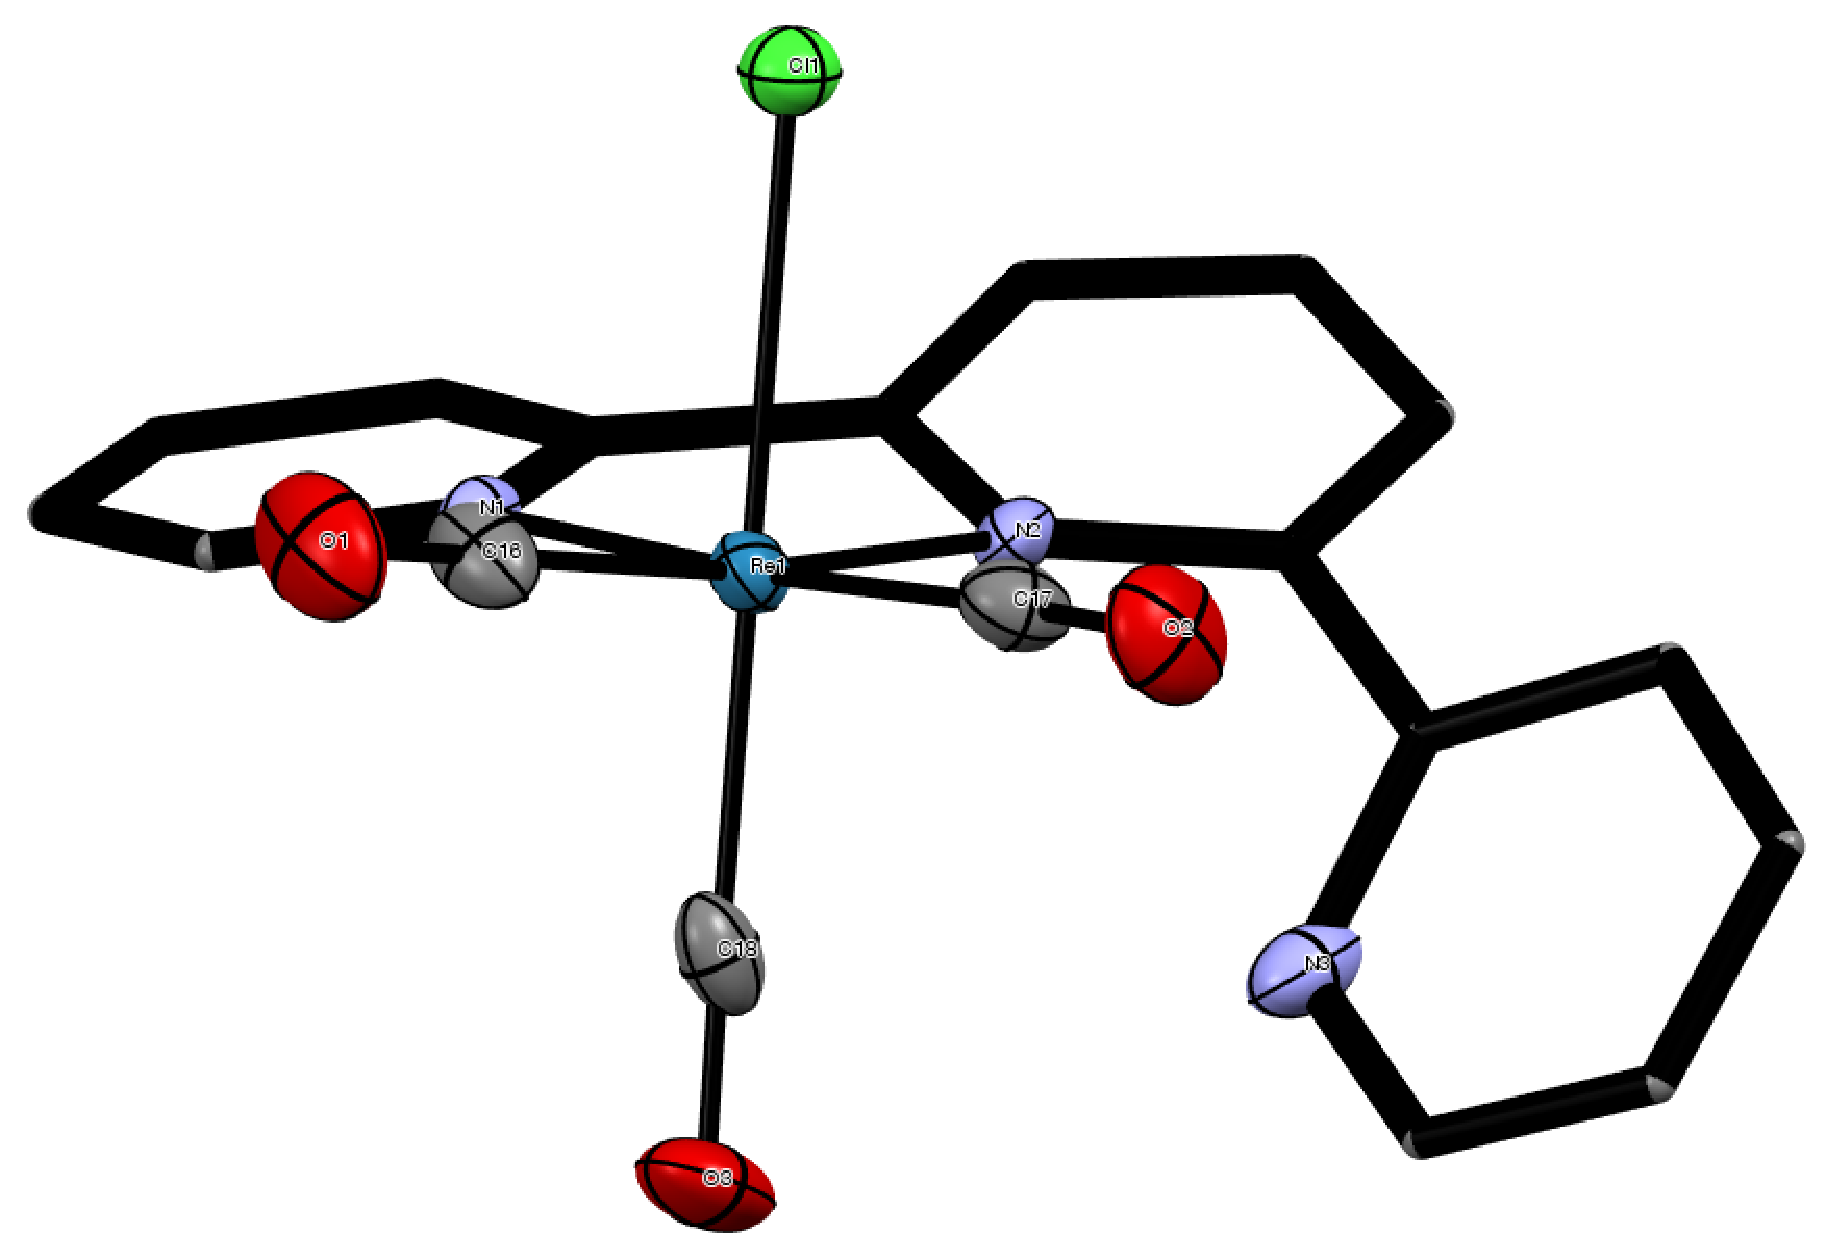
\includegraphics[clip=true, width=\textwidth, height=50mm, keepaspectratio]{images/xray1d.eps}
 \end{subfigure}
 \begin{subfigure}[b]{\textwidth}
  \centering
  \includegraphics[clip=true, width=\textwidth, height=75mm, keepaspectratio]{images/xray1uc.eps}
  \caption{Full unit cell representation of \textbf{2.1}}
 \end{subfigure}
\caption[X-ray crystal structure of \textbf{2.1}]{X-ray crystal structure of \textbf{2.1}. Co-crystallized chloroform, hydrogen atoms, and thermal ellipsoids of ligand carbon atoms are omitted for clarity.}
\label{fig.xray21}
\end{figure}

\begin{figure}[!ht]
 \centering
 \begin{subfigure}[b]{0.49\textwidth}
  \includegraphics[clip=true, width=\textwidth, height=50mm, keepaspectratio]{images/xray2a.eps}
 \end{subfigure}
 \begin{subfigure}[b]{0.49\textwidth}
  \includegraphics[clip=true, width=\textwidth, height=50mm, keepaspectratio]{images/xray2b.eps}
 \end{subfigure}
 \begin{subfigure}[b]{0.49\textwidth}
  \includegraphics[clip=true, width=\textwidth, height=50mm, keepaspectratio]{images/xray2c.eps}
 \end{subfigure}
 \begin{subfigure}[b]{\textwidth}
  \centering
  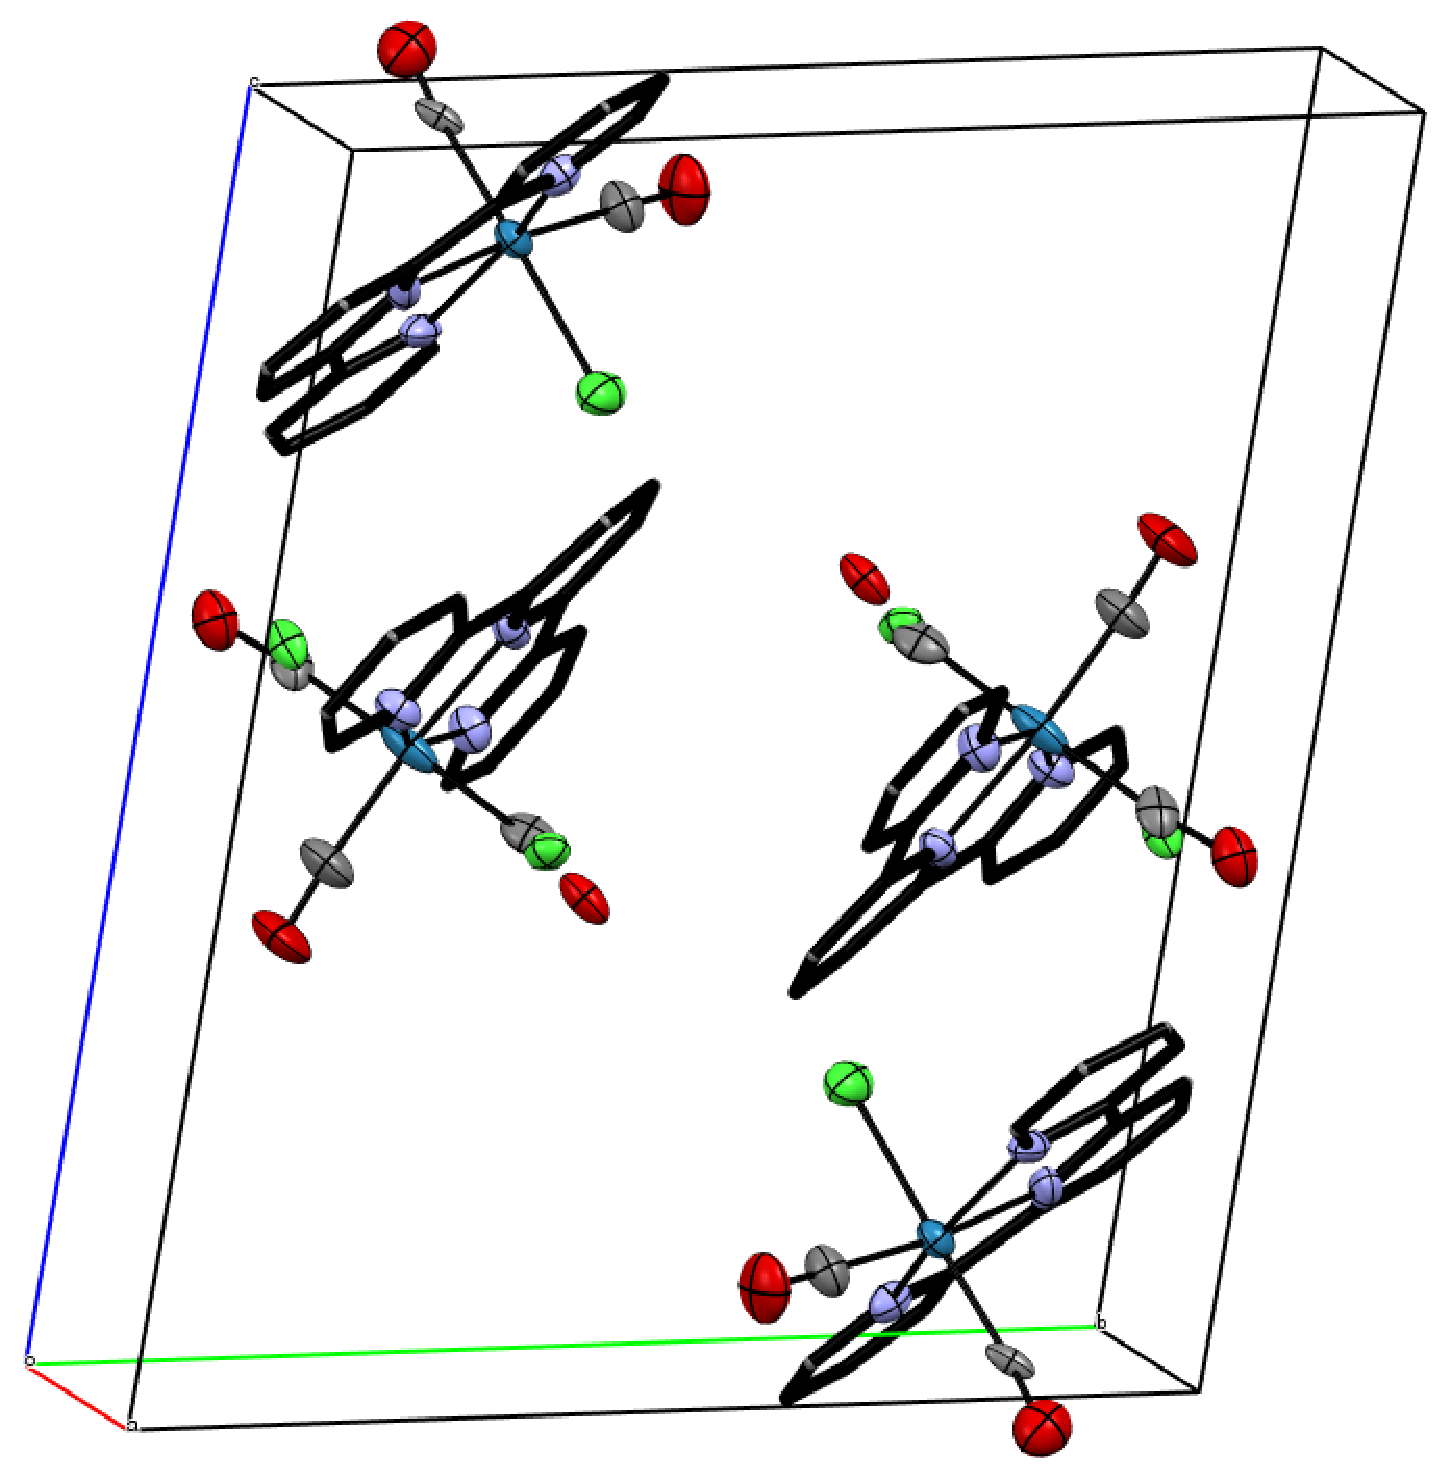
\includegraphics[clip=true, width=\textwidth, height=75mm, keepaspectratio]{images/xray2uc.eps}
  \caption{Full unit cell representation of \textbf{2.2}}
 \end{subfigure}
\caption[X-ray crystal structure of \textbf{2.2}]{X-ray crystal structure of \textbf{2.2}. Co-crystallized chloroform, hydrogen atoms, and thermal ellipsoids of ligand carbon atoms are omitted for clarity.}
\label{fig.xray22}
\end{figure}

\begin{figure}[!ht]
 \centering
 \begin{subfigure}[b]{0.49\textwidth}
  \includegraphics[clip=true, width=\textwidth, height=50mm, keepaspectratio]{images/xray3a.eps}
 \end{subfigure}
 \begin{subfigure}[b]{0.49\textwidth}
  \includegraphics[clip=true, width=\textwidth, height=50mm, keepaspectratio]{images/xray3b.eps}
 \end{subfigure}
 \begin{subfigure}[b]{0.49\textwidth}
  \includegraphics[clip=true, width=\textwidth, height=50mm, keepaspectratio]{images/xray3c.eps}
 \end{subfigure}
 \begin{subfigure}[b]{0.49\textwidth}
  \includegraphics[clip=true, width=\textwidth, height=50mm, keepaspectratio]{images/xray3d.eps}
 \end{subfigure}
 \begin{subfigure}[b]{\textwidth}
  \centering
  \includegraphics[clip=true, width=\textwidth, height=75mm, keepaspectratio]{images/xray3uc.eps}
  \caption{Full unit cell representation of \textbf{2.3}}
 \end{subfigure}
\caption[X-ray crystal structure of \textbf{2.3}]{X-ray crystal structure of \textbf{2.3}. Hydrogen atoms, and thermal ellipsoids of ligand carbon atoms are omitted for clarity.}
\label{fig.xray23}
\end{figure}

\begin{figure}[!ht]
 \centering
 \begin{subfigure}[b]{0.49\textwidth}
  \includegraphics[clip=true, width=\textwidth, height=50mm, keepaspectratio]{images/xray5a.eps}
 \end{subfigure}
 \begin{subfigure}[b]{0.49\textwidth}
  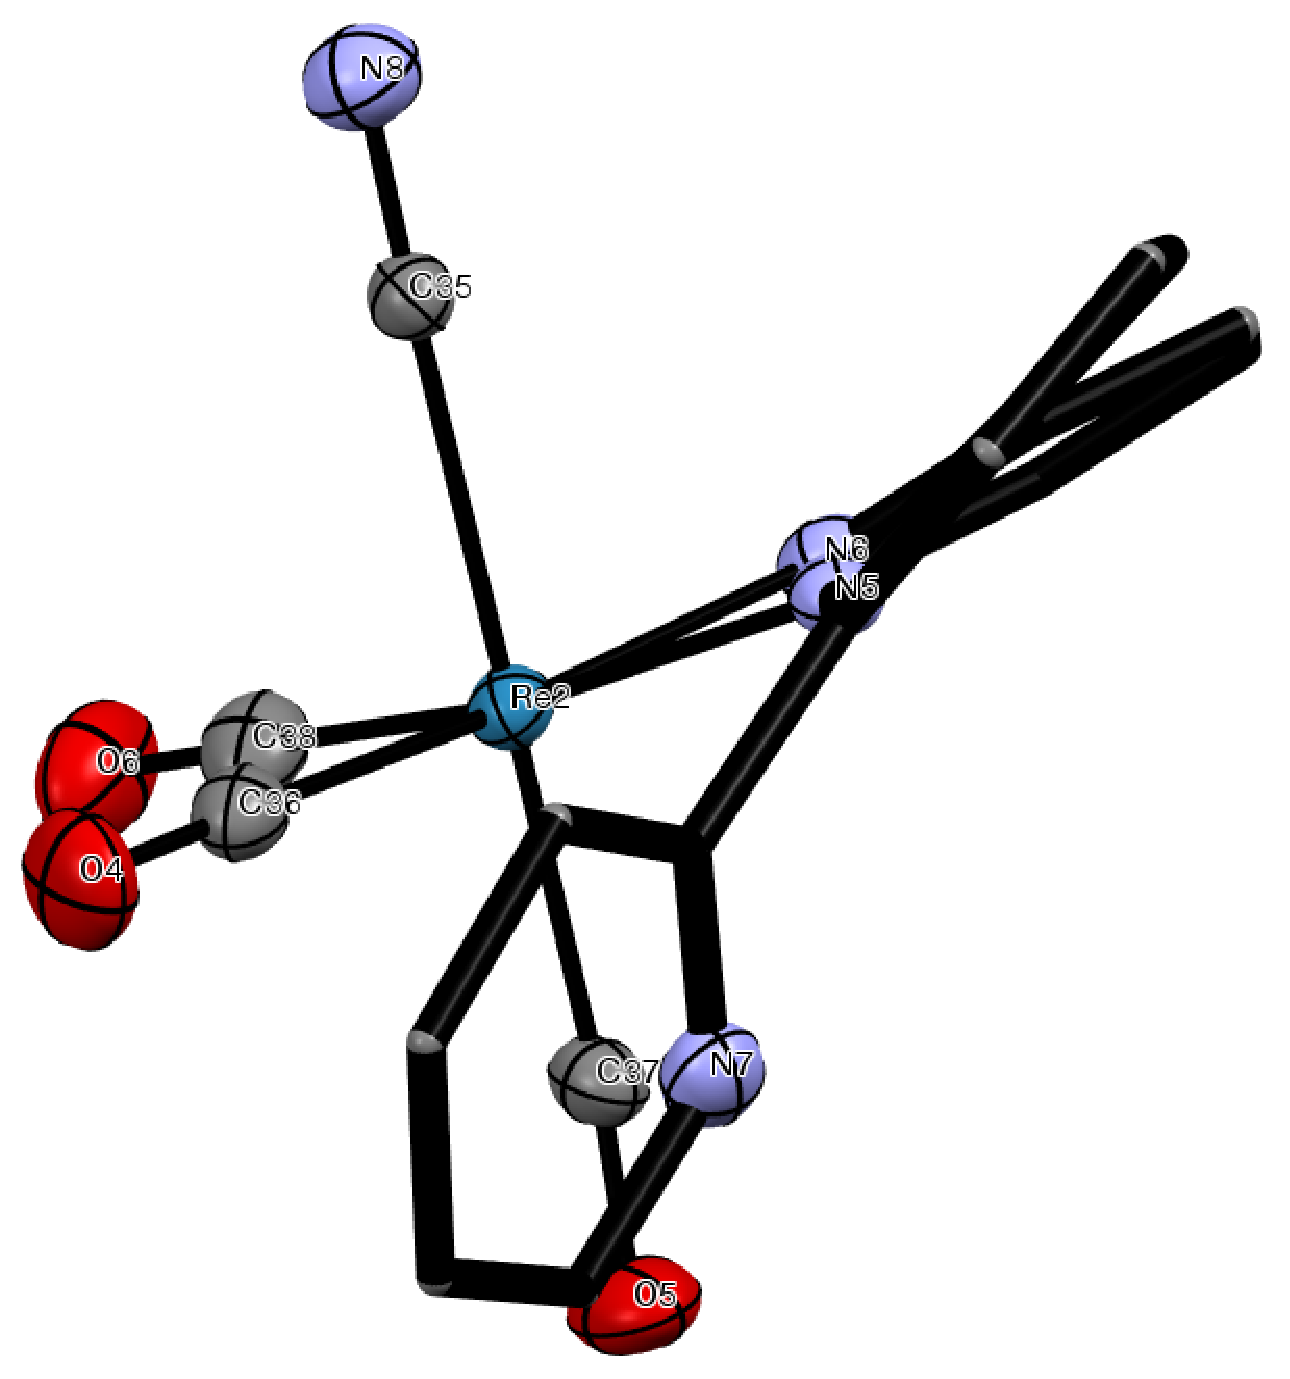
\includegraphics[clip=true, width=\textwidth, height=50mm, keepaspectratio]{images/xray5b.eps}
 \end{subfigure}
 \begin{subfigure}[b]{0.49\textwidth}
  \includegraphics[clip=true, width=\textwidth, height=50mm, keepaspectratio]{images/xray5c.eps}
 \end{subfigure}
 \begin{subfigure}[b]{0.49\textwidth}
  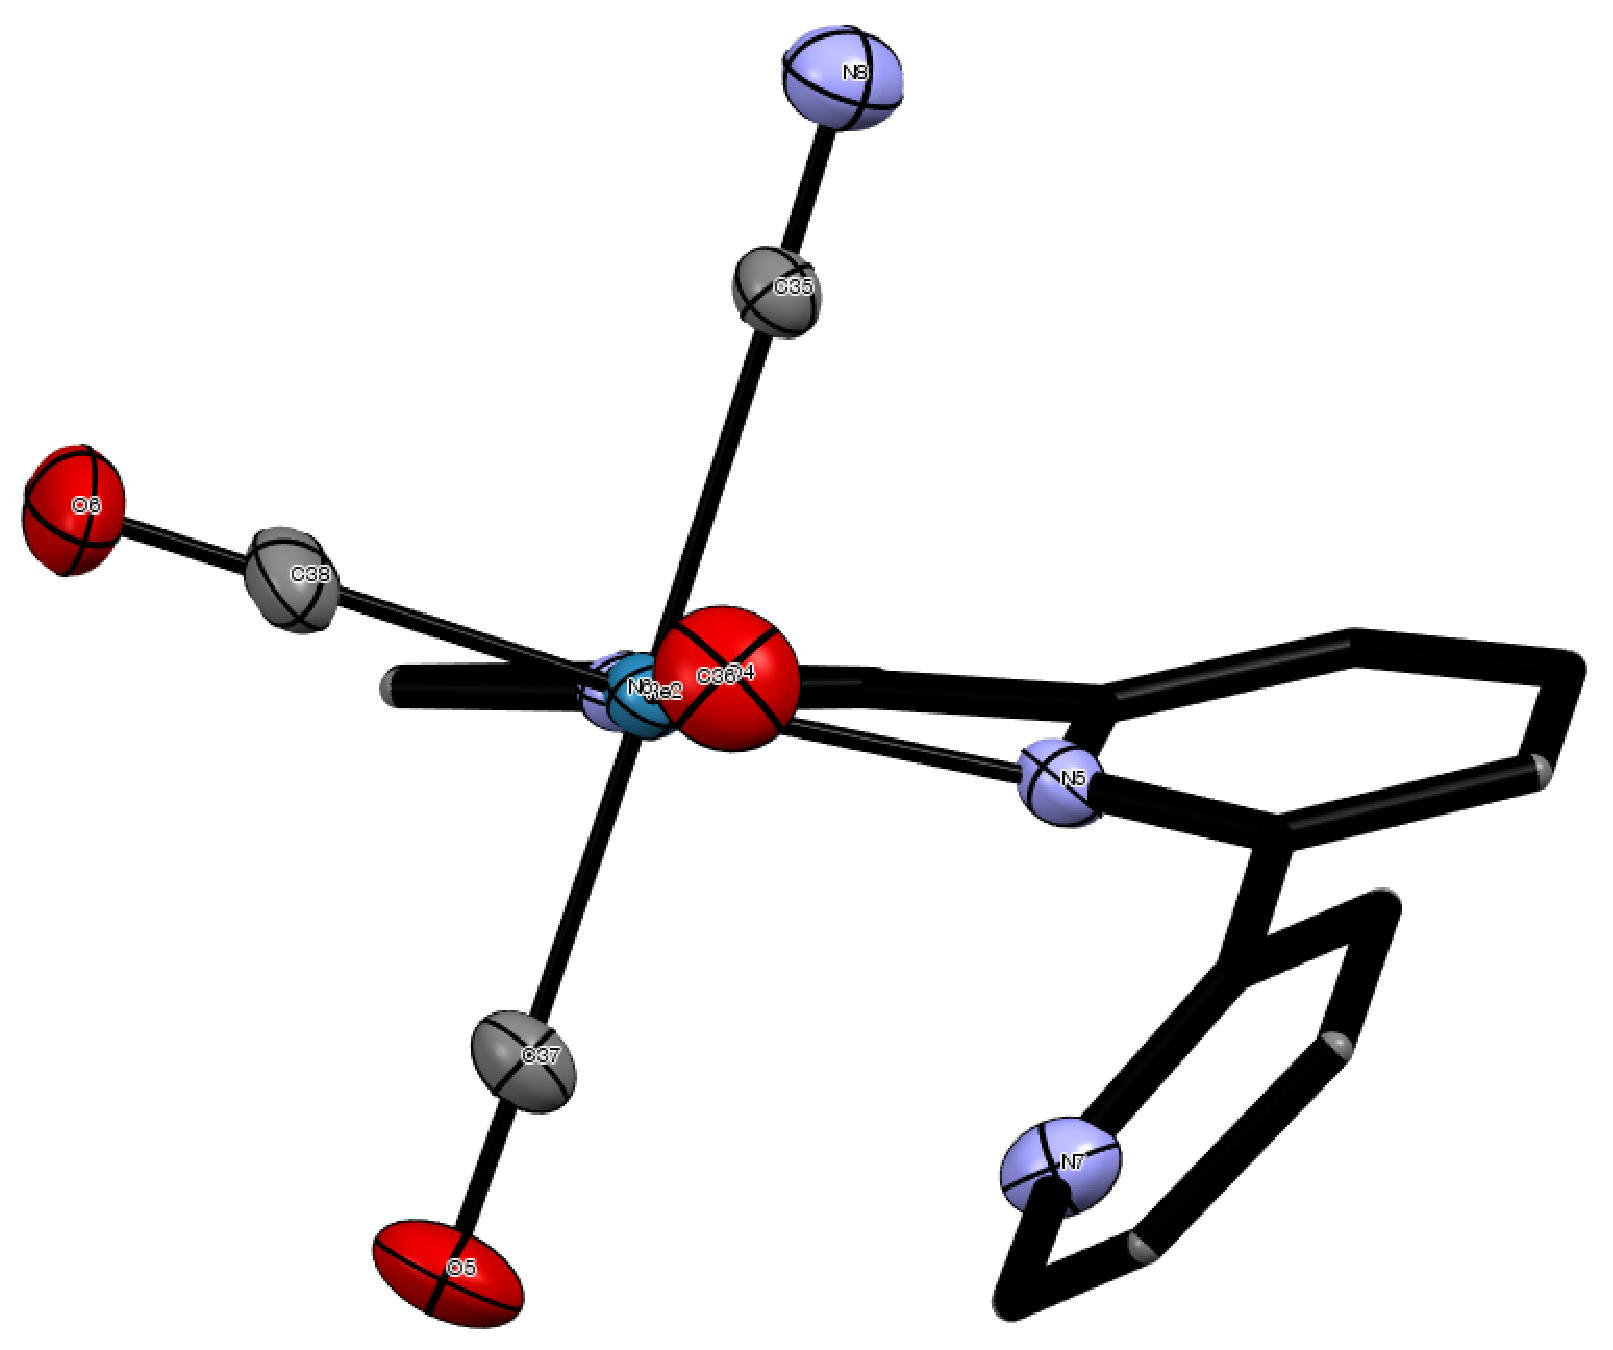
\includegraphics[clip=true, width=\textwidth, height=50mm, keepaspectratio]{images/xray5d.eps}
 \end{subfigure}
 \begin{subfigure}[b]{\textwidth}
  \centering
  \includegraphics[clip=true, width=\textwidth, height=75mm, keepaspectratio]{images/xray5uc.eps}
  \caption{Full unit cell representation of \textbf{2.5}}
 \end{subfigure}
\caption[X-ray crystal structure of \textbf{2.5}]{X-ray crystal structure of \textbf{2.5}. Hydrogen atoms, and thermal ellipsoids of ligand carbon atoms are omitted for clarity.}
\label{fig.xray25}
\end{figure}

\begin{figure}[!ht]
 \centering
 \begin{subfigure}[b]{0.49\textwidth}
  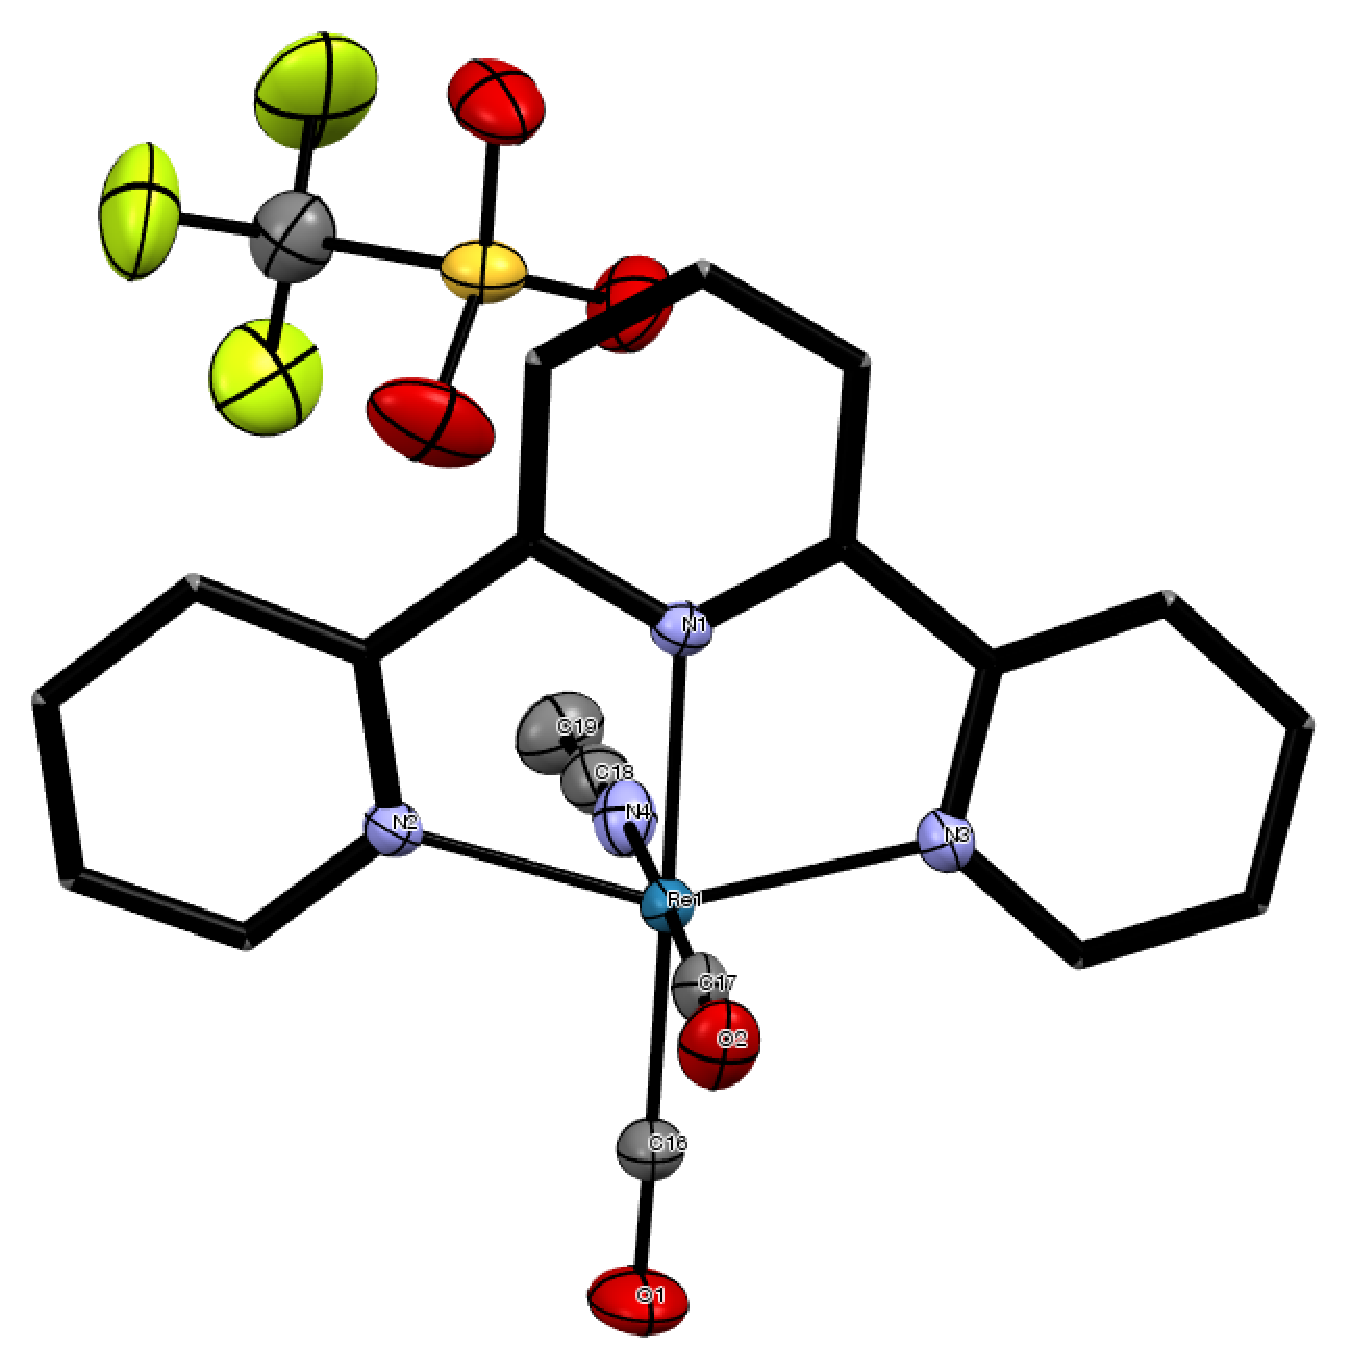
\includegraphics[clip=true, width=\textwidth, height=50mm, keepaspectratio]{images/xray8a.eps}
 \end{subfigure}
 \begin{subfigure}[b]{0.49\textwidth}
  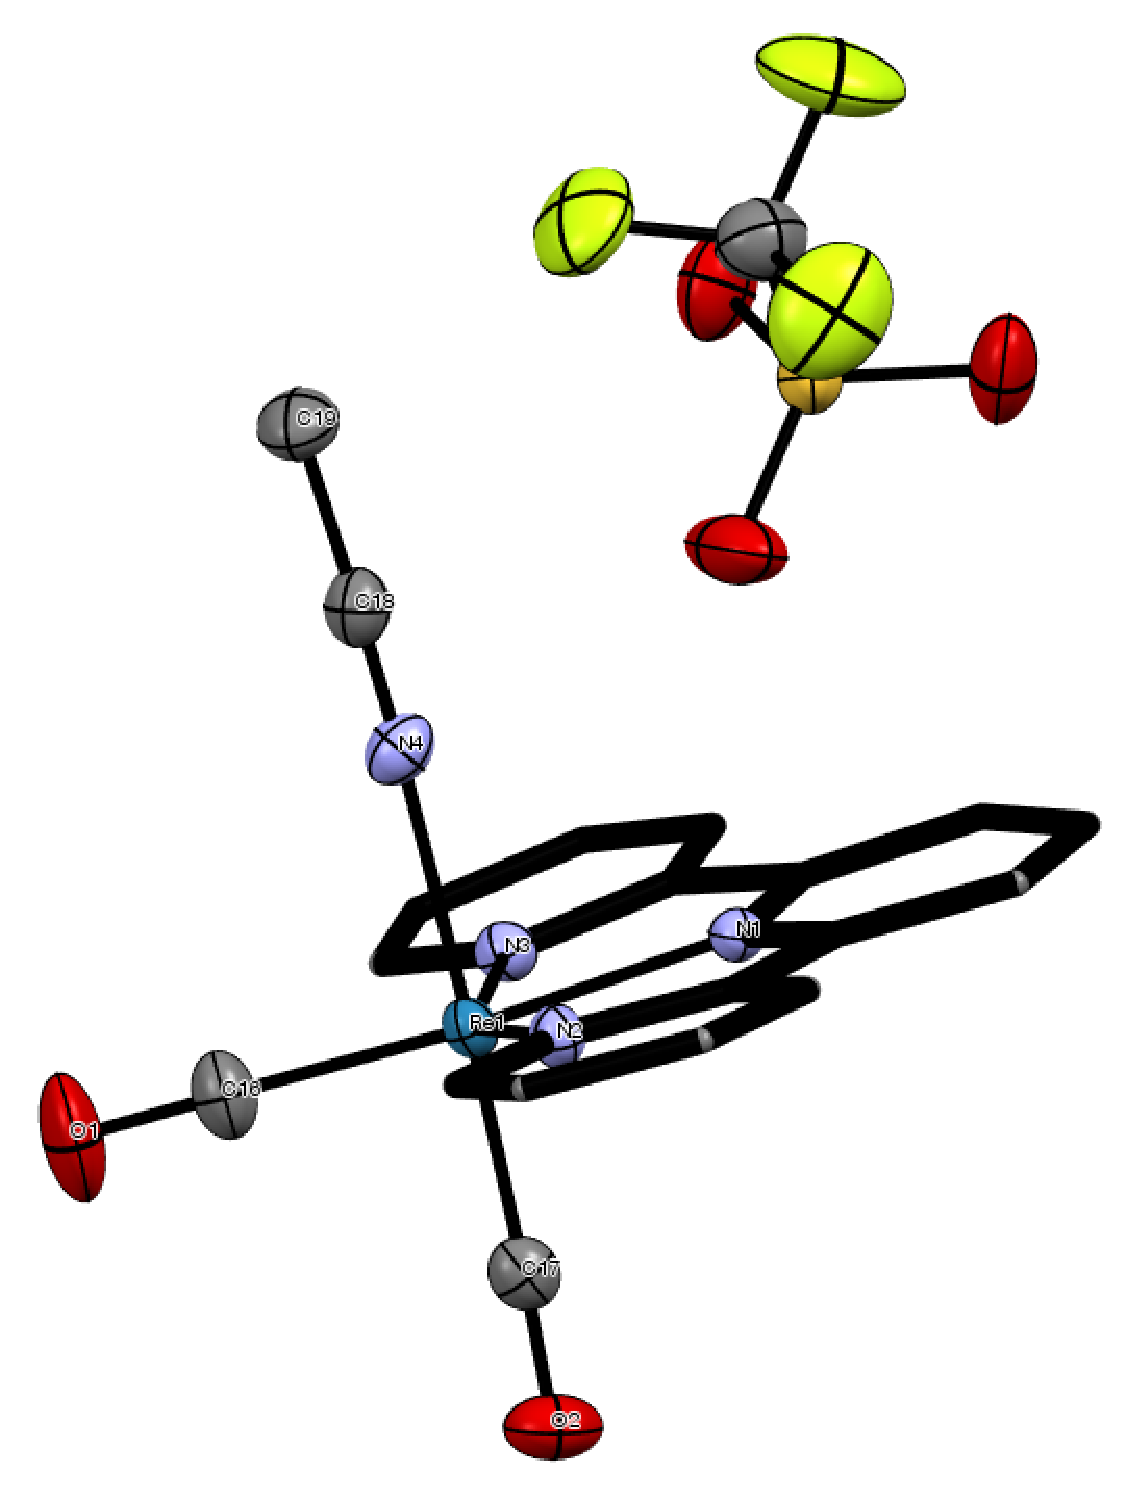
\includegraphics[clip=true, width=\textwidth, height=50mm, keepaspectratio]{images/xray8b.eps}
 \end{subfigure}
 \begin{subfigure}[b]{0.49\textwidth}
  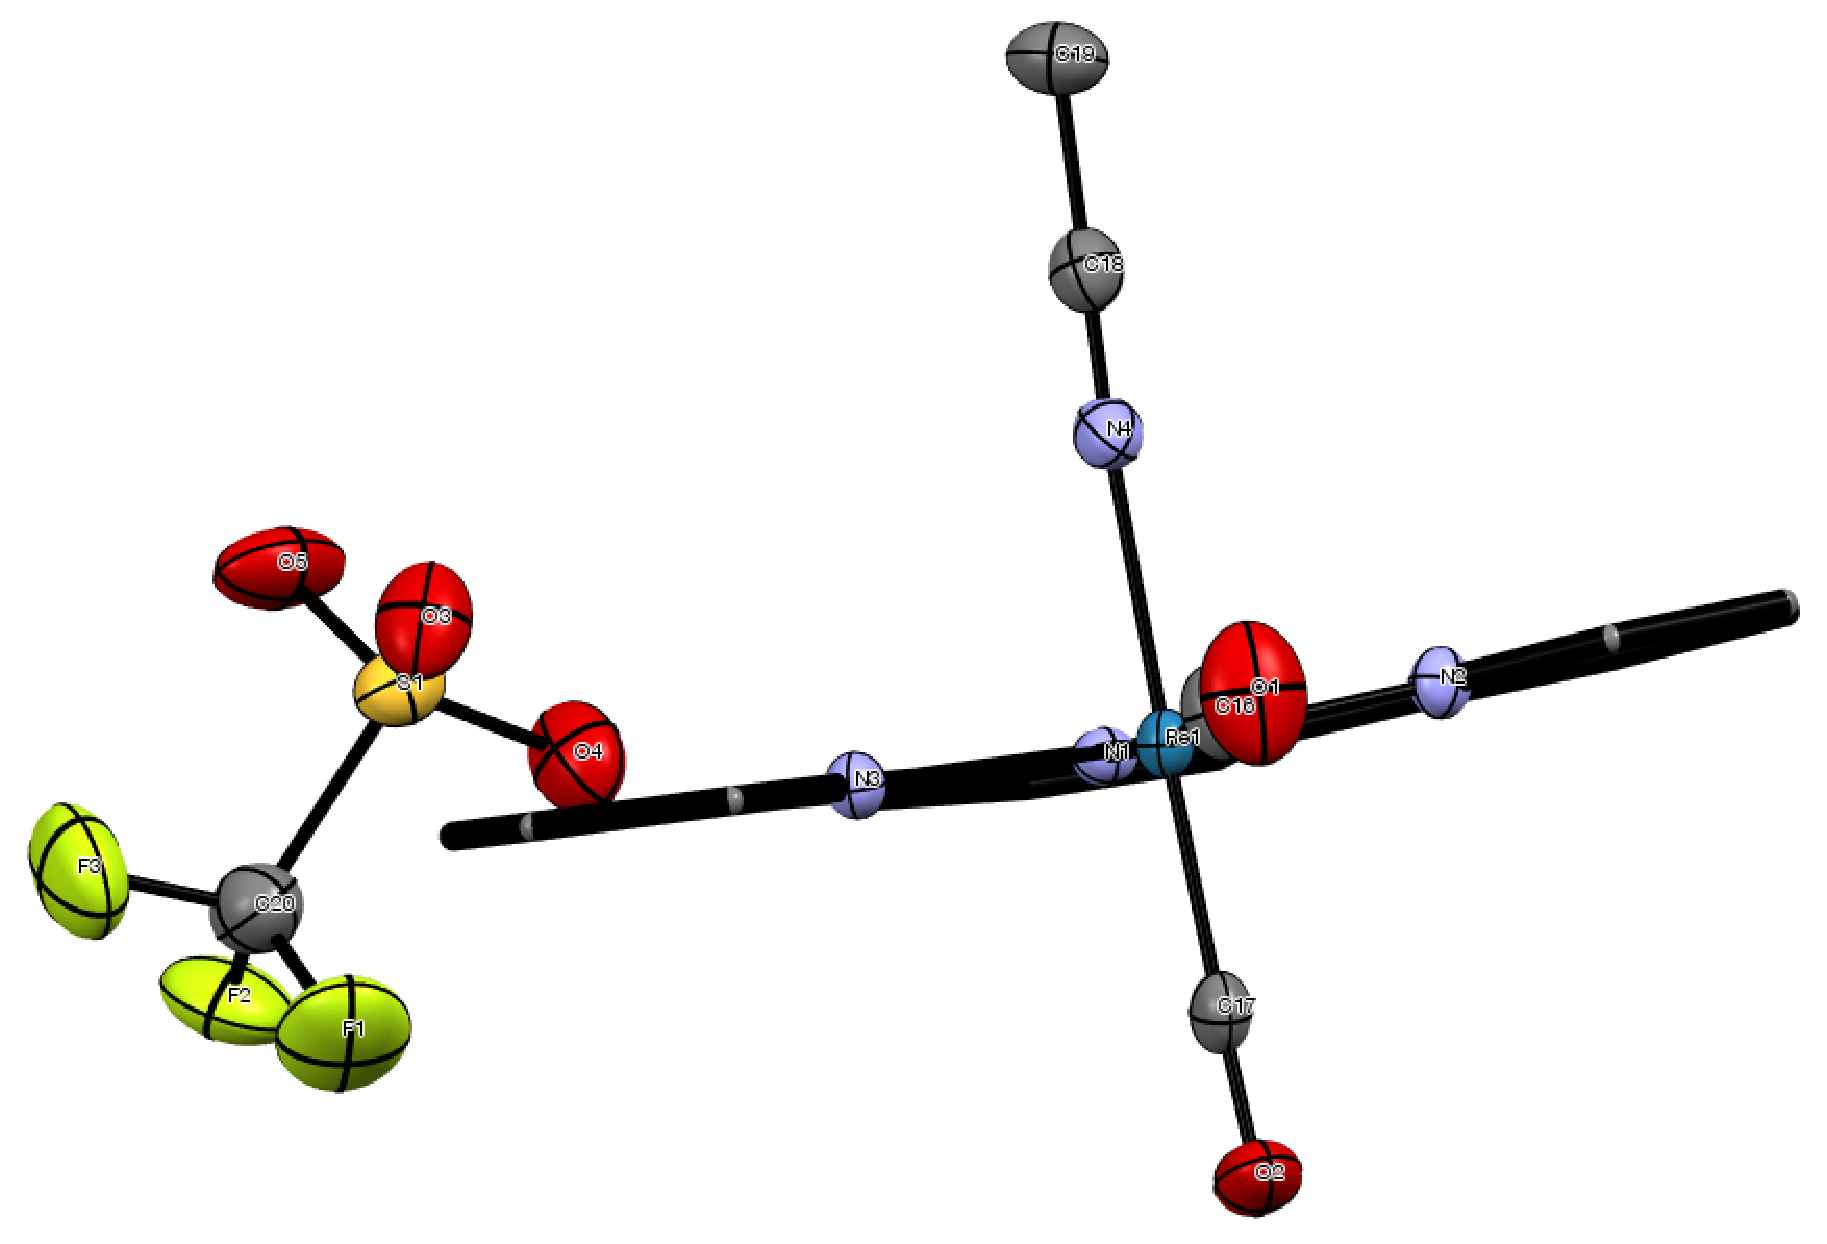
\includegraphics[clip=true, width=\textwidth, height=50mm, keepaspectratio]{images/xray8c.eps}
 \end{subfigure}
 \begin{subfigure}[b]{0.49\textwidth}
  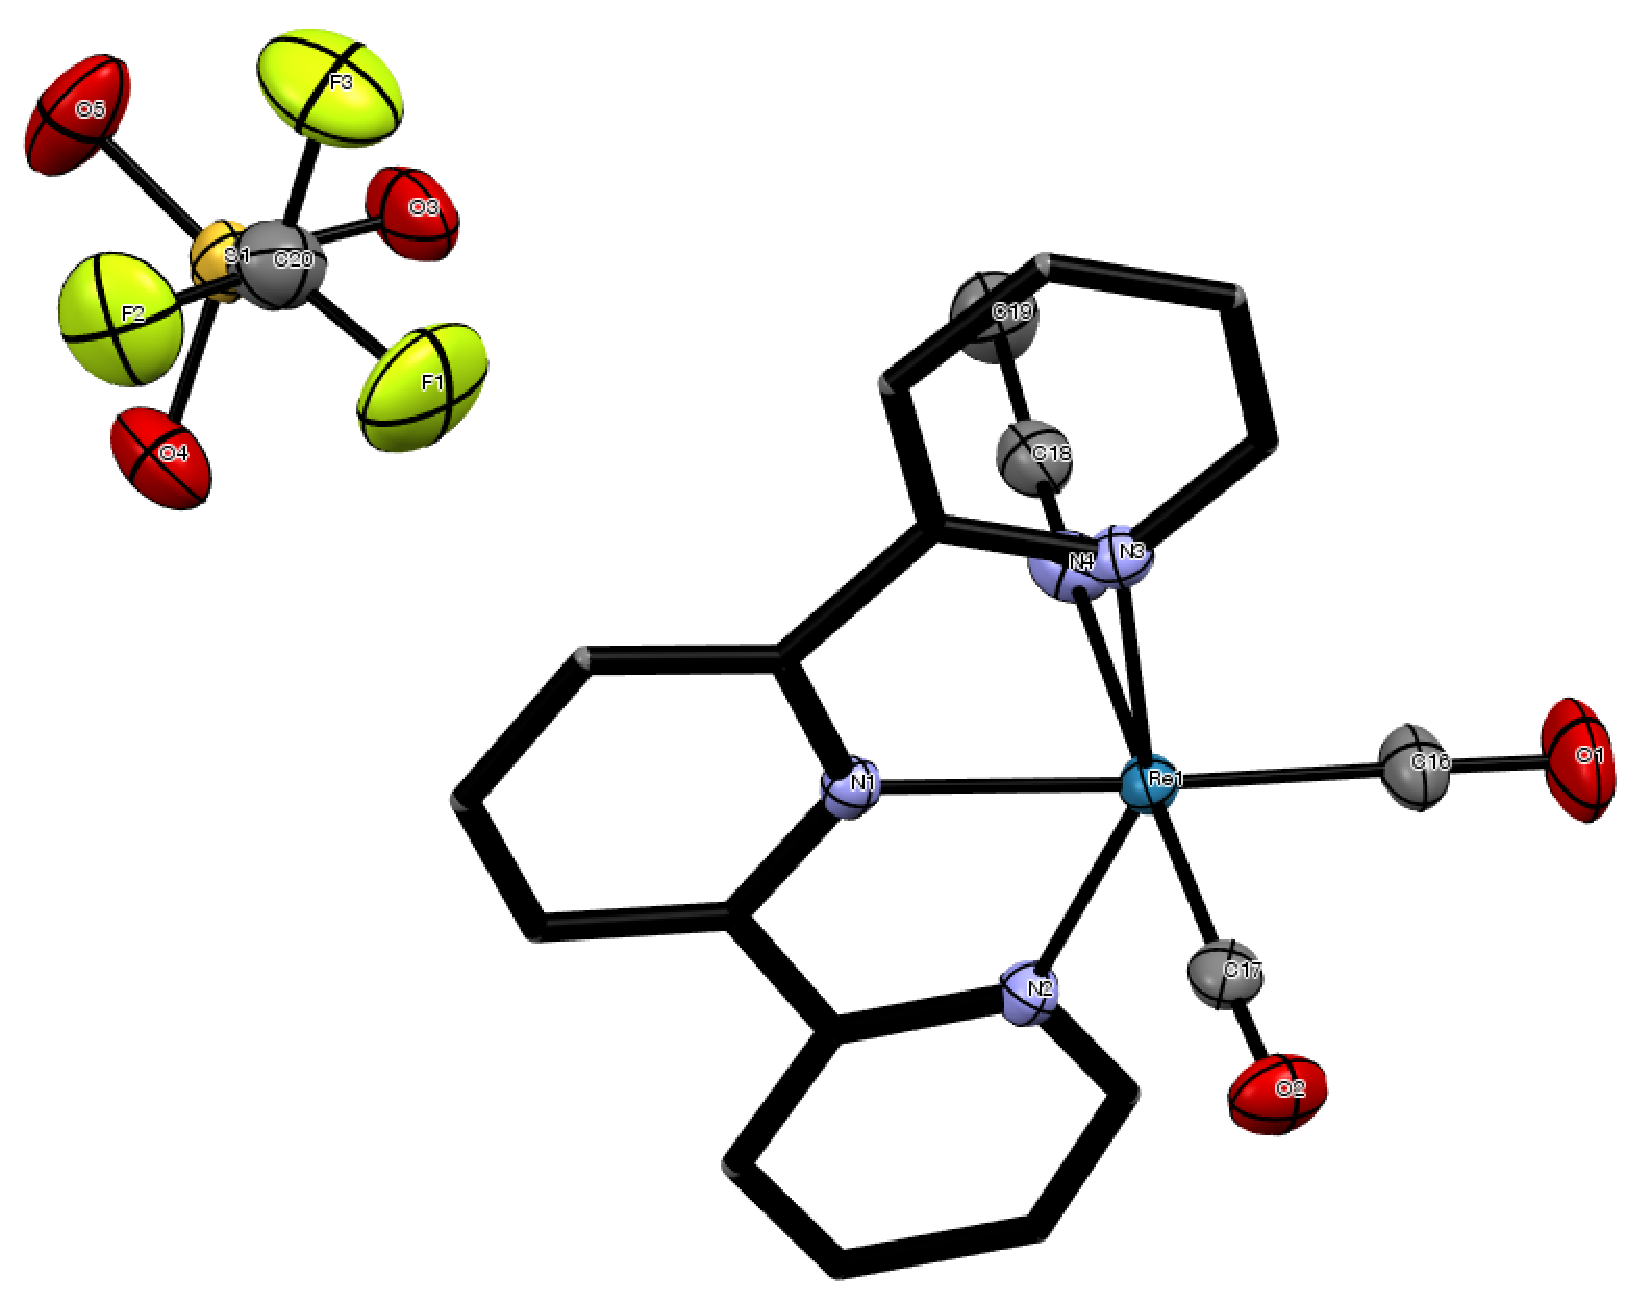
\includegraphics[clip=true, width=\textwidth, height=50mm, keepaspectratio]{images/xray8d.eps}
 \end{subfigure}
 \begin{subfigure}[b]{\textwidth}
  \centering
  \includegraphics[clip=true, width=\textwidth, height=75mm, keepaspectratio]{images/xray8uc.eps}
  \caption{Full unit cell representation of \textbf{2.8}}
 \end{subfigure}
\caption[X-ray crystal structure of \textbf{2.8}]{X-ray crystal structure of \textbf{2.8}. Hydrogen atoms, and thermal ellipsoids of ligand carbon atoms are omitted for clarity.}
\label{fig.xray28}
\end{figure}

\section{(terpy-$\kappa^2$-N,N$^\prime$)\ce{Re(CO)3Cl} (2.1)}\label{sec.c1}
\ce{Re(CO)5Cl} (201~mg,  0.556~mmol) and 2,2’:6’,2’’ terpyridine (129~mg, 0.553~mmol) were mixed in 60~mL of toluene. The reaction mixture was heated to 100°C for 1 hour under N2. During this time the solution turned a bright red. Upon cooling a yellow precipitate was formed. The solution was filtered, and the solid was washed with diethyl ether, and dried under vacuum. Compound \textbf{1} is a bright yellow powder that was isolated in 70~\% yield (208~mg). Crystals were obtained from chloroform with addition of a small amount of hexanes as counter solvent. TGA: 8~\% mass loss from 240-280~$^\circ$C.  FTIR: 2019, 1981, 1889 cm\ce{^{-1}} (\textit{v} C=O). \ce{^1H} NMR (\ce{CD3CN}, 400 MHz): $\delta$ 9.06 (ddd, J=5.6, 1.7, 0.8 Hz, 1H), 8.77 (ddd, J=4.9 Hz, 1H), 8.49 (td, J=8.2, 1.5 Hz, 2H), 8.28 (t, J=7.9 Hz, 1H), 8.22 (td, J=8.1, 1.6 Hz, 1H), 7.96 (td, J=7.8, 1.8 Hz, 1H), 7.79 (dt, J=7.8, 1.1 Hz, 1H), 7.80 (dd, J=7.7, 1.0 Hz, 1H), 7.63 (ddd, J=7.6, 5.5, 1.2 Hz, 1H), 7.55 (ddd, J=7.6, 5.0, 1.0 Hz, 1H). Elemental analysis calculated (\%) for [\ce{C18H11ReClN3O3}]: C 40.11, H 2.06, N 7.80, found C 39.96, H 2.09, N 7.69.

\section{(terpy-$\kappa^3$-N,N$^\prime$,N$^{\prime \prime}$)\ce{Re(CO)2Cl} (2.2)}\label{sec.c2}
Compound \textbf{1} (101~mg, 0.187~mmol) was placed in a tube furnace and heated to 240~$^\circ$C under \ce{N2} flow for 60 minutes. A black solid was collected (90~mg) at 94~\% yield based on the formula for \textbf{2}. Crystals were obtained from chloroform with addition of a small amount of hexanes as counter solvent. FTIR: 1872, 1788 cm\ce{^{-1}} (\textit{v} C=O). \ce{^1H} NMR (\ce{CD3CN}, 400 MHz): $\delta$ 8.70 (ddd, J=4.7, 1.8, 0.9 Hz, 2H), 8.65 (dt, J=8.0, 1.0, 1.0, 2H), 8.47 (d, J=7.8 Hz, 2H), 8.03 (t, J=7.8 Hz, 1H), 7.95 (td, J=7.7, 7.7, 1.9 Hz, 2H), 7.43 (ddd, J=7.5, 4.8, 1.2 Hz, 2H). Elemental analysis calculated (\%) for [\ce{C17H11ReClN3O2}]: C~39.96, H~2.17, N~8.22, found C~39.62, H~2.09, N~7.99.

\section{(terpy-$\kappa^2$-N,N$^\prime$)\ce{Re(CO)3Br} (2.3)}\label{sec.c3}
\ce{Re(CO)5Br} (191~mg, 470~mmol) and 2,2’:6’2’’ terpyridine (129~mg, 0.553~mmol) were allowed to react under conditions analogous to the preparation of \textbf{1}. A bright yellow powder was obtained, 0.223 g (0.382~mmol, 81~\%). FTIR: 2012, 1910, 1886 cm\ce{^{-1}} (\textit{v} C=O). \ce{^1H} NMR (\ce{CD3CN}, 400 MHz): $\delta$ 9.07 (ddd, J=5.6, 1.6, 0.9 Hz, 1H), 8.77 (ddd, J=4.6, 1.5, 0.8 Hz, 1H), 8.52 – 8.48 (m, 2H), 8.28 (t, J=7.9 Hz, 1H), 8.21 (td, J=8.0, 1.6 Hz, 1H), 7.97 (td, J=7.8, 1.8 Hz, 1H), 7.80 – 7.75(m, 2H), 7.63 (ddd, J=7.6, 5.5, 1.2 Hz, 1H), 7.55 (ddd, J=7.7, 4.9, 1.1 Hz, 1H). Elemental analysis calculated (\%) for [\ce{C18H11ReBrN3O3}]: C~37.06, H~1.90, N~7.20, found C~36.94, H~1.92, N~7.00.  

\section{(terpy-$\kappa^3$-N,N$^\prime$,N$^{\prime \prime}$)\ce{Re(CO)2Br} (2.4)}\label{sec.c4}
Compound \textbf{3} (182~mg, 0.312~mmol) was placed in an tube furnace and heated to 230~$^\circ$C under \ce{N2} flow for 60 minutes. A black solid was collected, 0.155~mg (0.279~mmol, 89~\% yield). Crystals were obtained from chloroform with addition of a small amount of hexanes as counter solvent. FTIR: 1873, 1794 cm\ce{^{-1}} (\textit{v} C=O). \ce{^1H} NMR (\ce{CD3CN}, 400 MHz): $\delta$ 8.95 (d, J=5.4 Hz, 2H), 8.24 (t, J = 8.1Hz, 4H), 8.05 (dd, J=8.2, 7.7 Hz, 1H), 7.90(td, J=7.9, 1.7 Hz, 2H), 7.63 (ddd, J=7.3, 5.5, 1.2 Hz, 2H). Elemental analysis calculated (\%) for [\ce{C17H11ReBrN3O2}]: C~36.76, H~2.00, N~7.57, found C~36.66, H~2.00, N~7.50.

\section{(terpy-$\kappa^2$-N,N$^\prime$)\ce{Re(CO)3CN} (3)} \label{sec.c5}
To \textbf{1} (80~mg, 0.148~mmol), \ce{AgCF3SO3} (46~mg, 0.179~mmol) was added in 10~mL \ce{CH2Cl2}. The reaction was stirred 18~h and kept dark under \ce{N2} atmosphere. Solution was filtered to remove salts, then reduced in volume. Cold diethyl ether was used to precipitate product. Yellow-grey powder (\textbf{7a}) was collected by filtration, yielding 38mg (40~\%). Crystals were grown from saturated chloroform with hexanes as countersolvent for X-ray crystallography. FTIR: 2013, 1905, 1884 cm\ce{^{-1}} (\textit{v} C=O). \ce{^1H} NMR (\ce{CD3CN}, 400 MHz): $\delta$ 9.08 (dd, J=5.40, 0.49 Hz, 1 H), 8.78 (dd, J=5.10, 0.59 Hz, 1 H), 8.53 (dd, J=8.18, 0.93 Hz, 1 H), 8.50 (d, J=8.23 Hz, 1 H), 8.30 (t, J=7.90 Hz, 1 H), 8.23 (td, J=7.94, 1.57 Hz, 2 H), 7.98 (td, J=7.76, 1.71 Hz, 1 H), 7.80 (dd, J=7.79, 1.03 Hz, 1 H), 7.77 (d, J=7.74 Hz, 0 H), 7.64 (ddd, J=7.50, 5.50, 1.08 Hz, 1 H), 7.55 (ddd, J=7.62, 4.92, 0.98 Hz, 2 H).  Elemental analysis calculated (\%) for [\ce{C19H11N4O3Re}]: C~43.10, H~2.09, N~10.58, found C~40.06, H~2.06, N~9.85.

\section{(terpy-$\kappa^3$-N,N$^\prime$,N$^{\prime \prime}$)\ce{Re(CO)2CN} (2.6)} \label{sec.c6}
To \textbf{2} (77~mg,  0.143~mmol), \ce{AgSO3CF3} (47~mg,  0.183~mmol) was added in 15~mL \ce{CH2Cl2}. Solution was stirred for 18~h in the dark under \ce{N2} atmosphere. Solution was filtered, then reduced to minimal volume. Cold diethyl ether was added dropwise to precipitate product. Collected by filtration and washed with additional cold ether, yielding 75~mg (120~mmol, 80~\%).  Crystals grown from saturated methylene chloride, with hexanes as countersolvent for x-ray crystallography. \ce{^1H} NMR (\ce{CD3CN}, 400 MHz): $\delta$ 8.60(ddt, J=4.8, 1.7, 0.8, 0.8 Hz, 2H), 8.48 (dq, J=8.0, 1.0 Hz, 2H), 8.37 (dd, J=7.9, 0.8 Hz, 2H), 8.07 (dd, J=8.0, 7.6 Hz, 1 H), 7.94 (ddd, J=7.9, 7.5, 1.8 Hz, 2H) 7.43 (ddd J=7.4, 4.8, 1.2 Hz, 2H). Elemental analysis calculated (\%) for [\ce{C18H11N4O2Re}]: C~43.11, H~2.21, N~11.17, found C~40.26, H~2.67, N~9.60.

\todo{CN Experimental, masses, \sout{ir}, \sout{nmr},  \sout{EA}}

\section{(terpy-$\kappa^2$-N,N$^\prime$)\ce{Re(CO)3OTf} (2.7)}\label{sec.c7}
To \textbf{1} (80~mg, 0.148~mmol), \ce{AgCF3SO3} (46~mg, 0.179~mmol) was added in 10~mL \ce{CH3CN}. The reaction was stirred 18~h and kept dark. Solution was filtered to remove salts, then reduced in volume. Cold diethyl ether was used to precipitate product. Yellow-grey powder (\textbf{7a}) was collected by filtration, yielding 38~mg (40~\%). Crystals were grown from saturated chloroform with hexanes as countersolvent for X-ray crystallography. FTIR: 2030, 1895, 1890 cm\ce{^{-1}} (\textit{v} C=O), 1280, 1228, 1204 cm\ce{^{-1}} (\textit{v} \ce{SO3}). \ce{^1H} NMR (\ce{CD3CN}, 400 MHz): $\delta$ 9.05 (ddd, J=5.5, 1.6, 0.8 Hz, 1H), 8.79 (ddd, J=4.9, 1.8, 1.1 Hz, 1H), 8.57 (dd, J=8.1, 0.9 Hz, 1H), 8.54 (dt, J=8.2, 1.1 Hz, 1H), 8.37 (t, J=7.9 Hz, 1H), 8.31 (td, J=8.0, 1.6 Hz, 1H), 8.03 (td, J=7.7, 1.7 Hz, 1H), 7.87 (dd, J=7.8, 1.0 Hz, 1H), 7.75 (dt, J=7.8, 1.1 Hz, 1H), 7.72 (ddd, J=7.4, 5.9, 1.1 Hz, 1H), 7.61 (ddt, J=7.7, 4.8, 0.5, 0.5 Hz, 1H).  Elemental analysis calculated (\%) for [\ce{C19H11ReN3O6F3S}]: C~34.97, H~1.70, N~6.44, found C~31.80, H~1.73, N~5.33.

Alternately, to \textbf{1} (72~mg, 0.134~mmol) was added 10~mL \ce{CF3SO3H} (excess) and temperature was increased to 100~$^\circ$C for 20 minutes. A black solution was neutralized with addition of 5\% \ce{Na2CO3} in \ce{H2O}. Product was extracted with \ce{CHCl3}, then dried under vacuum to yield a brown solid (\textbf{7b}) (47~mg, 54~\%).

\section{(terpy-$\kappa^3$-N,N$^\prime$,N$^{\prime \prime}$)\ce{Re(CO)2OTf} (2.8)}\label{sec.c8}
To \textbf{2} (77~mg,  0.143~mmol), \ce{AgSO3CF3} (47~mg,  0.183~mmol) was added in 15~mL \ce{CH3CN}. Solution was refluxed for 6~h in the dark under \ce{N2} atmosphere. Solution was filtered, then reduced to minimal volume. Cold diethyl ether was added dropwise to precipitate product. Collected by filtration and washed with additional cold ether, yielding 75~mg (120~mmol, 80~\%).  Crystals grown from saturated methylene chloride, with hexanes as countersolvent for x-ray crystallography. FTIR: 1910, 1829 cm\ce{^{-1}} (\textit{v} C=O), 1259, 1224, 1143 cm\ce{^{-1}} (\textit{v} \ce{SO3}). \ce{^1H} NMR (\ce{CD3CN}, 400 MHz): $\delta$ 8.91(ddd, J=5.6, 1.6, 0.7 Hz, 2H), 8.32 (d, J=8.0 Hz, 2H), 8.28 (ddd, J=8.1, 1.4, 0.8 Hz, 2H), 8.19 (dd, J=8.8, 7.4 Hz, 1H), 8.02 (td, J=7.9, 1.5 Hz, 2H) 7.46 (ddd J=7.6, 5.6, 1.3 Hz, 2H).  Elemental analysis calculated (\%) for [\ce{C18H11ReF3SN3O5}]: C~34.62, H~1.78, N~6.37, found C~31.02, H~1.82, N~7.11.



% An appendix
%======================================================================
\chapter{Molecular Orbitals and Energy Diagrams} \label{chap.mos}
\markright{Molecular Orbitals and Energy Diagrams}
%======================================================================

Frontier \glspl{ac.mo} for each compound discussed in this thesis are collected below. These orbitals are generated with the Chemissian program\autocite{chemissian}.

\missingfigure{Frontier \glspl{ac.mo} for \textbf{1}}

\begin{figure}[!htbp]
 \begin{center}
  \includegraphics[clip=true]{images/insertgraphic.eps}
 \end{center}
\caption{UV-Vis1}
\label{fig.uvvis1}
\end{figure}


\chapter{TurboControl and TurboGo Manual}\label{app.readme}
\markright{TurboControl User's Manual}


TurboControl is a series of scripts to run TurboMole jobs from Gaussian style inputs. The following is the user manual included with distributions of TurboControl 

\section{Introduction}
Gaussian software is well known for the user friendly GUI it contains (via GaussView). TurboMole, another computational suite, is known for its speed and optimizations, but has a significantly higher learning curve and is less beginner friendly. This software is an attempt to be able to use the user friendly input from Gaussian to smooth over the use of TurboMole.

\section{System Requirements}

There are two user-facing scripts available, both written to work with TurboMole 6.1-6.5 on clusters using Grid Engine queuing software. The only tests of operation are on a system with the following details:

\begin{itemize}
\itemsep1pt\parskip0pt\parsep0pt
\item
  Rocks 6.1 (Emerald Boa)/CentOS 6.3
\item
  Open Grid Scheduler/Grid Engine 2011.11p1
\item
  Python 2.7.3
\end{itemize}

Other systems, including different operating systems, different versions of Grid Engine or python, or on other systems, are not supported.

Python dependencies include:

\begin{itemize}
\itemsep1pt\parskip0pt\parsep0pt
\item
  pexpect 3.2\autocite{pexpect}
\item
  openbabel (optional)\autocite{openbabel, oboyle2011} 
\end{itemize}

Prior to running TurboGo or TurboControl, a valid installation of TurboMole must be available. On systems where computational modules must be loaded, TurboMole must have been loaded to the environment. Additionally, running the TurboMole environment configuration is recommended but not required prior to launching TurboGo or TurboControl:

\begin{center}
\begin{verbatim}
$ source $TURBODIR/Config_turbo_env
\end{verbatim}
\end{center}

\section{Installation}
Installation of TurboControl is very simple. Just extract the .tar.gz file available from the code repository at \url{https://github.com/pbulsink/turbocontrol/releases/latest}. Alternately, the source may be downloaded from \url{http://github.com/pbulsink/turbocontrol} and used without installation.

\section{TurboGo}

TurboGo is a script fun on an input file. It generates the inputs required for TurboMole jobs, and submits the job to the GridEngine queue before quitting. TurboGo is run with the following syntax:

\begin{center}
\begin{verbatim}
$ turbogo [-h] [-v] [-q] file
\end{verbatim}
\end{center}

positional arguments:

\begin{Verbatim}[baselinestretch=0.75]
file                  Read input from gaussian-type input FILE.
\end{Verbatim}

More info on the input files is available below.

optional arguments:

\begin{itemize}
\item \texttt{-h, --help            }Show this help message and exit
\item \texttt{-v, --verbose         }Run more verbose (show debugging info)
\item \texttt{-q, --quiet           }Run less verbose (show only warnings)
\end{itemize}

TurboGo saves a log file (turbogo.log) in the directory in which it is run. A second log file (define.log) will remain if the setup crashes or is terminated at some points, or if the script is run verbose.

TurboGo writes the final coordinates to final\_geometry.xyz. If openbabel is installed, it will also write finalgeom.mol. The entire optimization is written to optimization.xyz for viewing with a molecular viewer, such as vmd.

\section{TurboControl}

TurboControl is a management script called from a parent directory containing sub directories of input files. Each input file must be in its own directory. The input file format must be the same as the input format for TurboGo (listed above), with the extension `.in', `.inp', `.input', `.com', or `.gjf'. TurboControl reads the inputs and submits the jobs to the computational cluster queue. It then monitors running jobs to determine when the script has finished. If the job is an Opt-Freq, it prepares the frequency analysis and resubmits to the queue. TurboControl analyses completed Opt-Freq jobs for true optimization, and attempts to re-run jobs with modified geometries when Transition States are found. TurboControl will not get stuck on the same transition state, but will return a `stuck' job. TurboControl is run with the following syntax:

\begin{center}
\begin{verbatim}
$ turbocontrol [-h] [-v/-q] [-s]
\end{verbatim}
\end{center}

Optional arguments:

\begin{itemize}
\item \texttt{-h, --help            }Show this help message and exit
\item \texttt{-v, --verbose         }Run more verbose (show debugging info)
\item \texttt{-q, --quiet           }Run less verbose (show only warnings)
\item \texttt{-s, --solvent         }List available solvents for COSMO and quit
\end{itemize}

TurboControl outputs information every 3 hours on the status of the jobs. It writes a log file (\texttt{turbocontrol.log}) and may or may not leave other log files in each directory (depending on verbosity level). Ends when the last job finishes or crashes. Requires 1 node or can be run on the headnode (minimal resource consumption especially after initial job preparation and submission.)

TurboControl assists with analysis by outputting a \texttt{stats.txt} file as jobs complete. This file contains file details, optimization and frequency timing details, energy, and the first frequency. Additional information can be requested by including the \texttt{freeh} keyword (see below).

\section{Input File Format}

The input file format is similar to that well known by Gaussian users. A series of keywords, one per line and indicated by a `\%', is followed by the `route card' (specific job information). Charge and spin is indicated, then the molecule is shown in Cartesian format. This is followed by optional modifications to the TurboMole Control file. Note the location of blank lines in the example (Section 5.7).

\subsection{Keywords}

Keywords are as follows:

\begin{itemize}
\item \texttt{\%nproc} - number of processors to use for the calculation job.
  \begin{itemize}
    \item Synonym: \texttt{\%nprocessors}
  \end{itemize}
\item \texttt{\%arch} - parallelization architecture to use for the job.
  \begin{itemize}
    \item Synonyms: \texttt{\%architecture}, \texttt{\%para\_arch}
   \end {itemize}
\item \texttt{\%maxcycles} - number of optimization iterations before failing.
\item \texttt{\%autocontrolmod} - DEFAULT - modify the \texttt{control} file to include optimizations to speed up the job.
\item \texttt{\%nocontrolmod} - do not modify \texttt{control} file as above.
\item \texttt{\%rt} - specify max expected runtime (for any part of job)in hours. Allows backfilling in GridEngine queue to speed up job submission. For example, for a 1 hour opt and 4 hour freq, submit at least a \texttt{rt} of 4
\item \texttt{\%cosmo} - use TurboMole's COSMO solvation model with the specified solvent or \texttt{None} to use the idealized solvent (epsilon = infinity). List of available solvents can be shown by running \texttt{turbocontrol -s}
\end{itemize}

Gaussian args, including \texttt{\%nosave}, \texttt{\%rwf={[}file{]}}, \texttt{\%chk={[}file{]}}, and \texttt{\%mem={[}memory{]}} are silently ignored.

\subsection{Route Card Options}

Route cards take the form of the following:

\texttt{\# {[}jobtype(s){]} {[}joboption(s){]}}

Job types available:

\begin{itemize}
\item \texttt{opt} - Perform a geometry optimization
\item \texttt{freq} - Perform a frequency analysis. Specify method via numforce or aoforce. default = numforce
\item \texttt{sp} - Perform a single point energy calculation.
  \begin{itemize}
    \item Cannot be combined with Opt or Freq
  \end{itemize}
\item \texttt{ts} - Perform a transition state search to find 1 imaginary vibration. 
  \begin{itemize}
    \item Cannot be combined with Opt or Freq
  \end{itemize}
\item \texttt{prep} - Prepare the job but do not submit to queue.
  \begin{itemize}
    \item Cannot be combined with Opt or Freq
  \end{itemize}
\end{itemize}

Job options available:

\begin{itemize}
\item \texttt{ri} - Use TurboMole's ri approximation
\item \texttt{marij} - Use TurboMole's marij approximation 
  \begin{itemize}
    \item Requires \texttt{ri}
  \end{itemize}
\item \texttt{disp} - Use TurboMole's implementation of Grimme's dispersion, version 3
\item \texttt{aoforce} - Use aoforce for frequency jobs
\item \texttt{numforce} - Use numforce for frequency jobs
\item \texttt{freeh} - Use TurboMole's \texttt{freeh} thermodynamics data script to extract thermodynamic information after frequency analysis
\end{itemize}

\subsection{Title}

Following the Route cards, a blank line is added, then a line containing the title of the calculation. This can include any characters, spaces, etc., remaining on only one line. This is followed by a blank line.

\subsection{Charge and Spin}

Charge and spin are listed as two numbers separated by a space: charge spin (eg:0 1)

\subsection{Geometry}

Geometry in xyz coordinate format: Element xcoord ycoord zcoord. Z-matrix geometry is not supported by TurboControl or TurboGo.

\subsection{Additional control File Modifications}

Additional lines to be added or removed from control. Lines automatically added are, as required,:

\begin{Verbatim}[baselinestretch=0.75]
$ricore 0
$paroptions ga_memperproc 900000000000000 900000000000
$parallel_parameters  maxtask=10000
$ricore_slave 1
$maxcor 2048
\end{Verbatim}

Additional lines may be added, or lines removed, by placing them after the geometry with a \texttt{\$} (for addition) or \texttt{-\$} (for removal).

\subsection{Example Input File}

An example input file for benzene in dmf:

\begin{Verbatim}[baselinestretch=0.75]
%nproc=4
%arch=GA
%maxcycles=250
%rt=6
%cosmo=dmf
# opt freq b3-lyp/def2-TZVP ri marij numforce

Benzene Optimization & Frequency

0 1
C  0.000  1.396  0.000
C  1.209  0.698  0.000
C  1.209 -0.698  0.000
C  0.000 -1.396  0.000
C -1.209 -0.698  0.000
C -1.209  0.698  0.000
H  0.000  2.479  0.000
H  2.147  1.240  0.000
H  2.147 -1.240  0.000
H  0.000 -2.479  0.000
H -2.147 -1.240  0.000
H -2.147  1.240  0.000

$disp
-$paraoptions

\end{Verbatim}


\section{Code Details}\label{sec.code}

Coverage percentages of code unit tests are listed in \autoref{tab.codetest}. Results are low for def\_op, screwer\_op, cosmo\_op, freeh\_op, turbocontrol, and turbogo because they contain many lines of interacting with GridEngine or TurboMole. Testing is performed via monitoring the status of the scripts as they run in real conditions.

The code style is graded by PyLint and results are shown in \autoref{tab.pylint}. PyLint describes coding style, adherence to guidelines, and readability. It does not describe code efficiency or usefulness.

\begin{table}[!htb]
  \centering
    \caption{Test Coverage of scripts in TurboControl.}
    \begin{tabular}{crrrr}
    \toprule
    Name  & Statements & Missing & Excluded & Coverage \\
    \midrule
    cosmo\_op & 106   & 70    & 1     & 34\% \\
    cosmo\_op\_test & 17    & 1     & 0     & 94\% \\
    def\_op & 302   & 226   & 1     & 25\% \\
    def\_op\_test & 20    & 1     & 0     & 95\% \\
    freeh\_op & 162   & 55    & 1     & 66\% \\
    freeh\_op\_test & 27    & 1     & 0     & 96\% \\
    screwer\_op & 71    & 25    & 1     & 65\% \\
    screwer\_op\_test & 11    & 1     & 0     & 91\% \\
    test\_all & 18    & 0     & 0     & 100\% \\
    turbocontrol & 537   & 319   & 0     & 41\% \\
    turbocontrol\_test & 245   & 24    & 0     & 90\% \\
    turbogo & 343   & 132   & 0     & 62\% \\
    turbogo\_helpers & 383   & 52    & 0     & 86\% \\
    turbogo\_helpers\_test & 274   & 2     & 0     & 99\% \\
    turbogo\_test & 98    & 1     & 0     & 99\% \\ \midrule
    \textbf{TOTAL} & 2614  & 910   & 4     & 65\% \\
    \bottomrule
    \end{tabular}%
  \label{tab.codetest}
\end{table}%

\begin{table}[!htb]
  \centering
  \caption{PyLint Scores for Turbocontrol Code.}
    \begin{tabular}{cr}
    \toprule
    File  & Score /10 \\
    \midrule
    test\_all.py & 2.22 \\
    turbogo.py & 8.80 \\
    turbogo\_test.py & 6.97 \\
    turbocontrol.py & 8.55 \\
    turbocontrol\_test.py & 7.18 \\
    turbogo\_helpers.py & 8.81 \\
    turbogo\_helpers\_test.py & 7.45 \\
    def\_op.py & 8.18 \\
    def\_op\_test.py & 5.71 \\
    screwer\_op.py & 7.36 \\
    screwer\_op\_test.py & 6.67 \\
    freeh\_op.py & 8.71 \\
    freeh\_op\_test.py & 6.79 \\
    cosmo\_op.py & 8.22 \\
    cosmo\_op\_test.py & 6.67 \\
    \bottomrule
    \end{tabular}%
  \label{tab.pylint}
\end{table}%

\section{Citing TurboControl}

TurboControl, Turbogo, or any other parts of this code may be cited as:

Bulsink, Philip. TurboControl, v. 1.1.0. http://github.org/pbulsink/turbocontrol (accessed June 2014)

Change the version number to match the version that you used, and change the accessed date to when you installed or downloaded TurboControl. 

\section{License}

All third party software is a registered trademark of their respective creators. Use of third party software via this software is limited by the conditions as laid out by the respective companies. License to use this software in no way acts as a license to use any other separate referenced software.

The MIT License (MIT)

Copyright \copyright~2014 Philip Bulsink

Permission is hereby granted, free of charge, to any person obtaining a copy of this software and associated documentation files (the ``Software''), to deal in the Software without restriction, including without limitation the rights to use, copy, modify, merge, publish, distribute, sublicense, and/or sell copies of the Software, and to permit persons to whom the Software is furnished to do so, subject to the following conditions:

The above copyright notice and this permission notice shall be included in all copies or substantial portions of the Software.

THE SOFTWARE IS PROVIDED ``AS IS'', WITHOUT WARRANTY OF ANY KIND, EXPRESS OR IMPLIED, INCLUDING BUT NOT LIMITED TO THE WARRANTIES OF MERCHANTABILITY, FITNESS FOR A PARTICULAR PURPOSE AND NONINFRINGEMENT. IN NO EVENT SHALL THE AUTHORS OR COPYRIGHT HOLDERS BE LIABLE FOR ANY CLAIM, DAMAGES OR OTHER LIABILITY, WHETHER IN AN ACTION OF CONTRACT, TORT OR OTHERWISE, ARISING FROM, OUT OF OR IN CONNECTION WITH THE SOFTWARE OR THE USE OR OTHER DEALINGS IN THE SOFTWARE.


\singlespacing
% An appendix
%======================================================================
\label{chap.glos}
%======================================================================
\cleardoublepage
\printglossary



%glossary
% Bibliography 
% If done using the BibTeX program, use
%\bibliographystyle{style} % sorted alphabetically, labeled with numbers
%\bibliography{bibliography/thesis} % names file keylatex.bib as my bibliography file 
% OR, do it "by hand" inside a "thebibliography" enivironment
\printbibliography
\markright{List of To Dos} % new right header
\listoftodos
% Index 
% Put a \makeindex command in the Preamble if you use MakeIndex program
% and put 
% \printindex % here
% OR, do it "by hand" inside \begin{theindex} ... \end{theindex}
%----------------------------------------------------------------------
\end{document}
%======================================================================
